%\documentclass[handout]{beamer}
%\usepackage{pgfpages}
%\pgfpagesuselayout{4 on 1}[a4paper, landscape, border shrink=5mm]
%\pgfpageslogicalpageoptions{1}{border code=\pgfusepath{stroke}}
%\pgfpageslogicalpageoptions{2}{border code=\pgfusepath{stroke}}
%\pgfpageslogicalpageoptions{3}{border code=\pgfusepath{stroke}}
%\pgfpageslogicalpageoptions{4}{border code=\pgfusepath{stroke}}
\documentclass{beamer}
%\usetheme{nesl}  % Now it's a beamer presentation with the NESL theme!
\usetheme{Copenhagen}
\usepackage{tikz}
\usetikzlibrary{shapes,arrows}
\usepackage{url}
\usepackage{movie15}
\usepackage{verbatim}
\usefonttheme{serif}
\beamersetuncovermixins{\opaqueness<1>{25}}{\opaqueness<2->{15}}

% Make a new command that will make a new subsection and a frame with the same title
\newcommand{\fst}[2]{\subsection{#1}\frame{\frametitle{#1} #2}}

% Standard LaTeX stuff - note the optional abbreviated title being provided
\title[Developments of WRF 4D-Var]{Latest Developments of WRF 4D-Var}
\author[Zhang and Huang]{Xin Zhang \and
Xiang-Yu Huang}

\date{~\\
~\\
%~\\\tiny{12th WRF Users' Workshop, Boulder, CO}\\
  ~\\
  ~\\
  ~\\
 \tiny{NCAR is sponsored by the National Science Foundation}
}

\institute[NESL]{
% \url{xinzhang@ucar.edu} \\
   NCAR Earth System Laboratory \\
%  \url{ook@ucw.cz}\\
%  Charles University, Prague
}

% We want the NSF department logo
\logo{
\includegraphics[height=.25in]{NSF_NESL.jpg}}


\begin{document}

% The title page
\frame{\titlepage}

%%%%%%%%%%%%%%%%%%%%%%%%%
\begin{comment}
\section{Status of WRF 4D-Var V3.2}

\frame{
\frametitle{4D-Var versus 3D-Var\\(Adopted from ECMWF training Course 2008)}
\begin{itemize}
	\item 4D-Var is comparing observations with background model fields at the correct time \pause
	\item 4D-Var can use observations from frequently reporting stations \pause
	\item The dynamics and physics of the forecast model is in an integral part of 4D-Var, so observations are used in a meteorologically more consistent way \pause
	\item 4D-Var combines observations at different times during the 4D-Var window in a way that reduces analysis error \pause
	\item 4D-Var propagates information horizontally and vertically in a meteorologically more consistent way
\end{itemize}
}

\fst{WRF 4D-Var V3.2}{
\begin{itemize}
	\item WRF 4D-Var was firstly released in April, 2009 with V3.1. \pause
	\item WRF adjoint and tangent linear codes (WRFPLUS) were developed based on WRF V2.0.2 around 2005. \pause
	\item Multiple Program Multiple Data (MPMD) framework, needs 3 executables: WRFDA, WRFNL and WRFPLUS. \pause
	\item Simplified physical packages: surface drag, large scale condensation and a cumulus parameterization schemes ( Q. Xiao).\pause
	\item Weak constraint with digital filter.
\end{itemize}
}

\fst{Why upgrade ?}{
\begin{itemize}
	\item Numerous bug fixes, upgrades and improvements in WRF model since 2005. V3.3 was released.\pause
	\item Particularly, WRF infrastructure changes invalid some interfaces in WRFPLUS, such as the boundary variables can not be read in anymore.\pause
	\item MPMD WRF 4D-Var is too complicate, most of the community users could not get it run without help. \pause
	\item Very high disk IO overhead associated with the number of processors.\pause
	\item Only runs good on IBM machines; unstable on other platforms and compilers.\pause
	\item Hard to do a complete adjoint check due to initial design of framework.
\end{itemize}
}
\end{comment}

%%%%%%%%%%%%%%%%%%%%%%%%%%%%%%%%%
\section{What's new}

\fst{New WRFPLUS V3.3.1}{
\begin{itemize}
   	\item New WRF tangent linear and adjoint codes (WRFPLUS V3.3.1) based on the latest WRF repository codes. \pause
	\item WRFPLUS V3.3.1 can be used as a standalone tool , such as in application of forecast sensitivity to observation and observation impact. \pause
	\item Accurate tangent linear and adjoint check. \pause
	\item WRF model, WRF tangent linear model and adjoint model are compiled as a library and callable subroutines in WRFDA framework. \pause
	\item Customized coupler to couple WRFDA, WRF and WRFPLUS as a single executable system. \pause 
	\item Robust WRF 4D-Var system across various  platforms and compilers ( IBM, Linux, Mac : xlf, pgi, intel, gfortran, g95). 
\end{itemize}
}

\begin{frame}[fragile]
\frametitle{Sample Tangent Linear and Adjoint Check of WRFPLUS }
\setbeamercolor{postit}{fg=black, bg=yellow}
\begin{beamerboxesrounded}[ lower=postit,shadow=true]{Tangent linear check:6 hours}
{\tiny
\begin{verbatim}
alpha_m=.1000E+00  coef=   0.98186174930325E+00  val_n= 0.3725210E+11  val_l= 0.3794027E+11
alpha_m=.1000E-01  coef=   0.99807498026522E+00  val_n= 0.3786723E+09  val_l= 0.3794027E+09
alpha_m=.1000E-02  coef=   0.99970559707666E+00  val_n= 0.3792910E+07  val_l= 0.3794027E+07
alpha_m=.1000E-03  coef=   0.99992019503144E+00  val_n= 0.3793724E+05  val_l= 0.3794027E+05
alpha_m=.1000E-04  coef=   0.10000447262220E+01  val_n= 0.3794196E+03  val_l= 0.3794027E+03
alpha_m=.1000E-05  coef=   0.99999981575068E+00  val_n= 0.3794026E+01  val_l= 0.3794027E+01
alpha_m=.1000E-06  coef=   0.99999998152933E+00  val_n= 0.3794027E-01  val_l= 0.3794027E-01
alpha_m=.1000E-07  coef=   0.99999990980017E+00  val_n= 0.3794026E-03  val_l= 0.3794027E-03
alpha_m=.1000E-08  coef=   0.99999956711797E+00  val_n= 0.3794025E-05  val_l= 0.3794027E-05
alpha_m=.1000E-09  coef=   0.10000030220656E+01  val_n= 0.3794038E-07  val_l= 0.3794027E-07
alpha_m=.1000E-10  coef=   0.99996176999678E+00  val_n= 0.3793882E-09  val_l= 0.3794027E-09
\end{verbatim}
}
\end{beamerboxesrounded}
\pause
\begin{beamerboxesrounded}[ lower=postit,shadow=true]{Adjoint check: 6 hours}
{\tiny
\begin{verbatim}
 ad_check: VAL_TL:    0.42476489986911E+11
 ad_check: VAL_AD:    0.42476489986912E+11
\end{verbatim}
}
\end{beamerboxesrounded}
\end{frame}

\begin{comment}
\fst{Single observation experiment}{
\begin{itemize}
	\item Initial time: $2000\_01\_25\_00:00:00$
	\item Ending time: $2000\_01\_25\_06:00:00$
	\item Observation: 500 mb temperature at {\color{red}ending time} \\
	          $O-B=-1.168K$
	\item Plotting the difference at {\color{red}ending time} between the forecast from analysis and from background to investigate the impact of 6h obs. on IC.
\end{itemize}
}

\frame{
\begin{columns}[c]
\column{5cm}
\includemovie[
  controls,poster={single/centernolbcjcdf.pdf},
  text={\large(Click to start the movie)\hspace*{400pt}}
]{6.0cm}{7.5cm}{single/centernolbcjcdf.mpeg}
\column[c]{3.5cm}
\begin{block}{Remarks}
\tiny{Forecasted 500mb T difference \\(DA forecast - reference forecast)}
\begin{itemize}
	\item {\color{red}$\star$} is the location of obs. at the ending time (6h).
	\item \tiny{Initial perturbation is on the upstream of the obs.}
	\item \tiny{Evolved perturbation at 6h hit the obs. location}
\end{itemize}
\end{block}
\end{columns}
}

\frame{
\begin{columns}[c]
\column{5cm}
\includemovie[
  controls,poster={centernolbcjcdf.pdf},
  text={\large(Click to start the movie)\hspace*{400pt}}
]{6.0cm}{7.5cm}{centernolbcjcdf.mpeg}
\column[c]{3.5cm}
\begin{block}{Remarks}
\tiny{Forecasted 500mb T difference \\(DA forecast - reference forecast)}
\begin{itemize}
	\item {\color{red}$\star$} is the location of obs. at the ending time (6h).
	\item \tiny{LBC control is  {\color{red}turned off}}
	\end{itemize}
\end{block}
\end{columns}
}

\frame{
\frametitle{What we learn:}
\begin{itemize}
	\item WRF 4D-Var has the capability to assimilate the observations within a time window.
	\item WRF 4D-Var produces the flow-dependent analysis increments.
\end{itemize}
}
\end{comment}

\fst{Lateral boundary condition control}{
\begin{equation*}
J=J_b+J_o+J_c+\color{red}J_{lbc}
\end{equation*}
\begin{eqnarray*}
J_{lbc} & = & \frac{1}{2}(\mathbf{x}(t_k)-\mathbf{x}_b(t_k))^T\mathbf{B}^{-1}(\mathbf{x}(t_k)-\mathbf{x}_b(t_k))\\
& = & \frac{1}{2}\delta\mathbf{x}(t_k)^T\mathbf{B}^{-1}\delta\mathbf{x}({t_k})
\end{eqnarray*}
$J_{lbc}$ is the $J_b$ at the end of the assimilation window and the
lateral boundary control is obtained through
\begin{eqnarray*}
\frac {\partial{\delta{\mathbf{x}}_{lbc}}} {\partial{t}}=\frac{\delta\mathbf{x}(t_k)-\delta\mathbf{x}(t_0)}{t_k-t_0}
\end{eqnarray*}
}

\frame{
\frametitle{Single observation experiment}
To investigate the impact of lateral boundary control, the 6h observation is placed close to boundary and downstream of the boundary inflow, we expect that the major analysis increments at 0h should be in boundary condition and outside of domain.
}

\frame{
\begin{columns}[c]
\column{5cm}
\includemovie[
  controls,poster={single/boundarynolbcjcdf.pdf},
  text={\large(Click to start the movie)\hspace*{400pt}}
]{6.0cm}{7.5cm}{single/boundarynolbcjcdf.mpeg}
\column[c]{3.5cm}
\begin{block}{Remarks}
\tiny{Forecasted 500mb T difference \\(DA forecast - reference forecast)}
\begin{itemize}
	\item {\color{red}$\star$} is the location of obs. at the ending time (6h).
	\item \tiny{LBC control is {\color{red}turned off}}
\end{itemize}
\end{block}
\end{columns}
}

\frame{
\begin{columns}[c]
\column{5cm}
\includemovie[
  controls,poster={single/boundarylbcjcdf.pdf},
  text={\large(Click to start the movie)\hspace*{400pt}}
]{6.0cm}{7.5cm}{single/boundarylbcjcdf.mpeg}
\column[c]{3.5cm}
\begin{block}{Remarks}
\tiny{Forecasted 500mb T difference \\(DA forecast - reference forecast)}
\begin{itemize}
	\item {\color{red}$\star$} is the location of obs. at the ending time (6h).
	\item \tiny{$O-B=-0.95K$}
	\item \tiny{LBC control is {\color{red}turned on}}
\end{itemize}
\end{block}
\end{columns}
}

\frame{
\frametitle{What we learn:}
\begin{itemize}
	\item The major increment is in the boundary condition( south boundary, invisible here)
	\item There is almost no increment in initial condition.
	\item For observations close to in-flow boundary, the impact of LBC control is important.
\end{itemize}
}

\begin{comment}
\subsection{Single executable 4D-Var}
\begin{frame}[fragile]
\frametitle{Single executable 4D-Var}
WRFPLUS includes WRF NL, AD and TL model and they are used as a subroutine in WRF 4D-Var, other than being called via shell scripts.
~\\
~\\
\setbeamercolor{postit}{fg=black, bg=yellow}
\begin{beamerboxesrounded}[ lower=postit,shadow=true]{Nonlinear call}
\begin{verbatim}
old         call da_system ("da_run_wrf_nl.ksh")
new         call da_nl_model
\end{verbatim}
\end{beamerboxesrounded}
\begin{beamerboxesrounded}[ lower=postit,shadow=true]{Tangent linear call}
\begin{verbatim}
old         call da_system ("da_run_wrfplus_tl.ksh")
new         call da_tl_model
\end{verbatim}
\end{beamerboxesrounded}
\begin{beamerboxesrounded}[ lower=postit,shadow=true]{Adjoint call}
\begin{verbatim}
old         call da_system ("da_run_wrfplus_ad.ksh")
new         call da_ad_model
\end{verbatim}
\end{beamerboxesrounded}
\end{frame}

\begin{frame}[fragile]
\frametitle{Memory exchange}
The information (TL perturbation, adjoint forcing, basic states and gradient) is exchanged via linked lists.
~\\
~\\
\setbeamercolor{postit}{fg=black, bg=yellow}
\begin{beamerboxesrounded}[ lower=postit,shadow=true]{Read basic states}
\begin{verbatim}
call domain_clock_get( grid, current_timestr=timestr )
call da_read_basicstates ( xbx, grid, ... )
\end{verbatim}
\end{beamerboxesrounded}
\begin{beamerboxesrounded}[ lower=postit,shadow=true]{Save TL perturbation}
\begin{verbatim}
call push_tl_pert (timestr)
\end{verbatim}
\end{beamerboxesrounded}
\begin{beamerboxesrounded}[ lower=postit,shadow=true]{Save AD forcing}
\begin{verbatim}
call push_ad_forcing (timestr)
\end{verbatim}
\end{beamerboxesrounded}
\end{frame}
\end{comment}

\subsection{Parallel performance}
\frame{
\frametitle{WRF 4D-Var V3.2: Parallel run using part of processors}
4D-Var is a sequential algorithm. However, the old WRF 4D-Var constructed on the Multiple Program Multiple Data mode, which have to split the total processors into 3 subsets for DA, NL and AD/TL. Lots of CPU time are wasted
\begin{center}
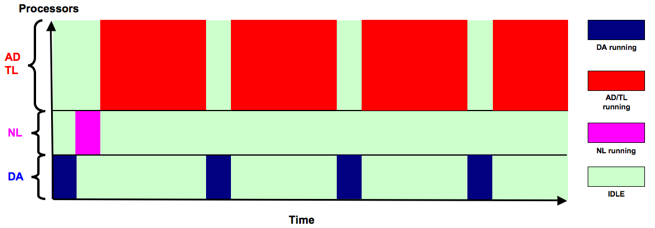
\includegraphics[scale=0.5]{mpmd_wrf4dvar}
\end{center}
}

\frame{
\frametitle{WRF 4D-Var V3.3.1: Parallel run using all processors}
Benefit from the single executable framework, every CPU is working at any time. No IDLE any more.
\begin{center}
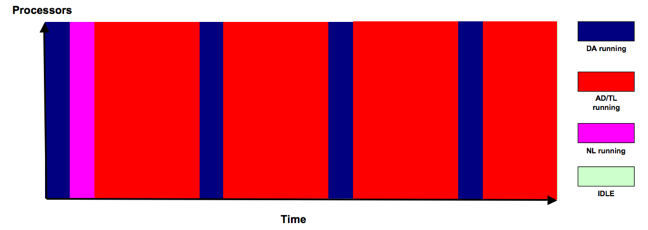
\includegraphics[scale=0.5]{single_exe_wrf4dvar}
\end{center}
}

\frame{
\frametitle{Performance improvement WRF 4D-Var framework}
\begin{itemize}
	\item $270x180x41@20km$,6h window, 1h obs\_bin, 10 iterations
	\item 10 iterations FGAT (identity TL/AD model), NCAR bluefire (IBM P6)
\end{itemize}
\begin{center}
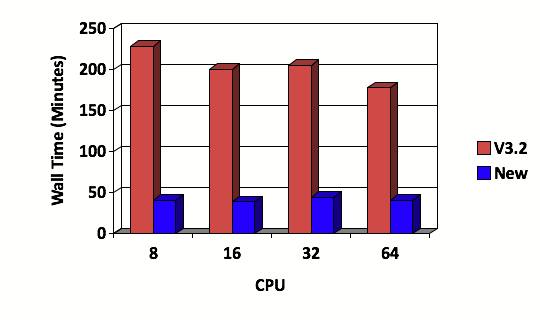
\includegraphics[scale=0.5]{big_case_performance}
\end{center}
}

\frame{
\frametitle{Parallel Strategies for WRFPLUS}
\begin{itemize}
	\item Modify registry tools and add the capability to generate tangent linear and adjoint codes for halo exchanges. 
	\item Add �halo\_nta� identifier in registry entry to instruct registry to automatically generate tangent linear and adjoint code for some halo exchange stencils.
\end{itemize}
}

\frame{
\frametitle{Parallel timing/speedup of WRF NLM/TLM/ADM}
Domain size: 350x250x57L, 27km\\
On IBM bluefire,  xlf V13.01, per time step \\ 
~\\
~\\
\begin{tabular}{c | c | c | c | c}
\hline
Processors & Perfect & NLM & TLM & ADM \\
\hline \hline
8 & 1 & 4.06s/1.0 & 8.14s/1.0 & 22.06s/1.0 \\
16 & 2 & 2.14s/1.90 & 4.27s/1.91 & 11.37s/1.94 \\
32 & 4  & 1.09s/3.72  & 2.17s/3.75 & 5.89s/3.74 \\
64 & 8 & 0.63s/6.44 & 1.21s/6.73 & 3.25s/6.79 \\
128 & 16 & 0.32s/12.69 & 0.62s/13.13 & 1.75s/12.61\\
256 & 32 & 0.32s/12.69 & 0.44s/18.50 &1.28s/17.23 \\
\hline
\end{tabular}
}

\frame{
\frametitle{Parallel timing/speedup of WRF NLM/TLM/ADM}
Domain size: 700x500x41L, 15km\\
On IBM bluefire,  xlf V13.01, per time step \\ 
~\\
~\\
\begin{tabular}{c | c | c | c | c}
\hline
Processors & Perfect & NLM & TLM & ADM \\
\hline \hline
64 & 1 & 1.57s/1.0 & 3.22s/1.0 & 7.69s/1.0 \\
128 & 2 & 0.82s/1.91 & 1.61s/2.0 & 4.27s/1.80 \\
256 & 4 & 0.71s/2.21 & 1.30s/2.48 & 3.95s/1.94 \\
512 & 8 & 0.39s/4.03 & 0.61s/5.28 & 1.83s/4.20 \\
1024 & 16 & 0.24s/6.54 & 0.34s/9.47 & 0.91s/8.45 \\
\hline
\end{tabular}
}

\begin{comment}

\subsection{Multi-increment regrid strategy}
\frame{
\frametitle{Multi-increment regrid strategy}
\begin{itemize}
	\item Fine grid to coarse grid: Decimation 
	\begin{itemize}
		\item There are 114 variables 
			\begin{itemize}
				\item 1D variables (43), 2D variables (51 ), 3D variables(20)
				\item 1D variables are constants or profiles, no necessary to make decimation
			\end{itemize}
		\item All variables except 1D variables
		\item The thinning grids have the same geographical coordinate with the coarse grids generated by real
		\item The thinning girds are consistent with the coarse grids generated by real
		\item The thinning grids are very close the coarse grids generated by real
	\end{itemize}
	\item Coarse grid to Fine grid: Bilinear Interpolation
		\begin{itemize}
			 \item Increments regridded 
				\begin{itemize}
					\item U,V,T,QVAPOR,PH,P
					\item MU,PSFC,Q2,T2,TH2,U10,V10
				\end{itemize}
		\end{itemize}
\end{itemize}
}

\frame{
\frametitle{Flow chart of Multi-incremental 4D-Var}
\begin{center}
\includegraphics[scale=0.45]{multi-inc}
\end{center}
}

\end{comment}

\begin{comment}
\frame{
\frametitle{Performance improvement WRF 4D-Var framework}
\begin{itemize}
	\item $90x60x41@60km$, 6h window, 1h obs\_bin
	\item 27 iterations FGAT, NCAR bluefire (IBM P6)
\end{itemize}
\begin{center}
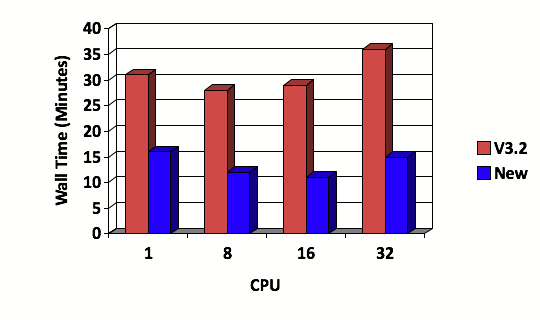
\includegraphics[scale=0.5]{small_case_performance}
\end{center}
}
\end{comment}

\begin{comment}
\fst{Weak constraint with digital filter (enhanced)}{
\begin{tabular}{l p{2in}}
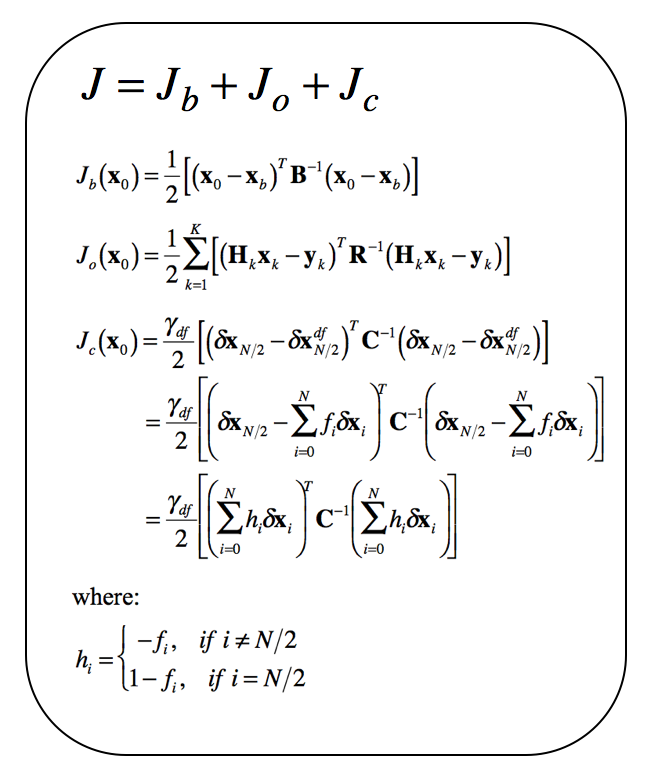
\includegraphics[scale=0.25]{jcdf_formular} \pause & 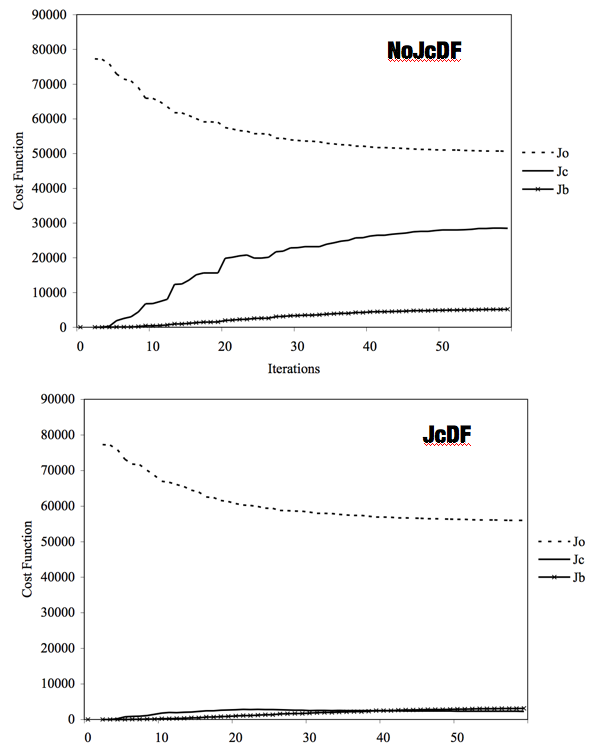
\includegraphics[scale=0.25]{jcdf}
\end{tabular}
}

\frame{
\frametitle{Weak constraint with digital filter \\(domain averaged surface pressure variation) }
\begin{center}
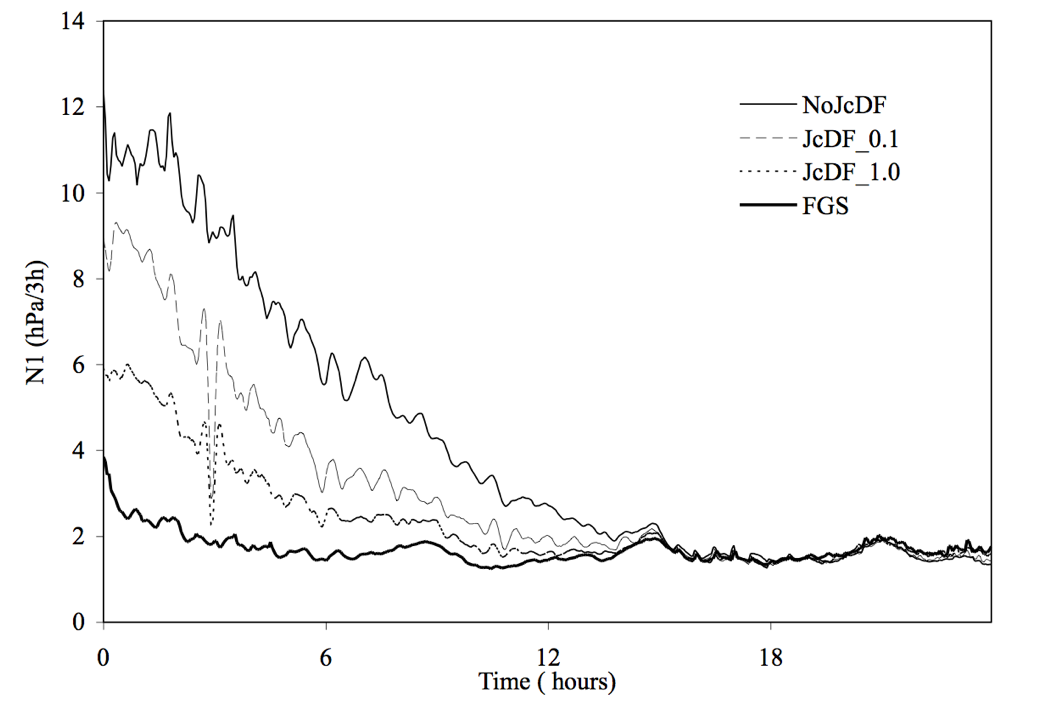
\includegraphics[scale=0.25]{jcdf_ps}
\end{center}
}
\end{comment}

\begin{comment}
\fst{Observations used by 4D-Var}{
\begin{itemize}
	\item Conventional observational data (little\_r, prepbufr)
	\item Radar radial velocity
	\item Radiance satellite data
\end{itemize}
\begin{center}
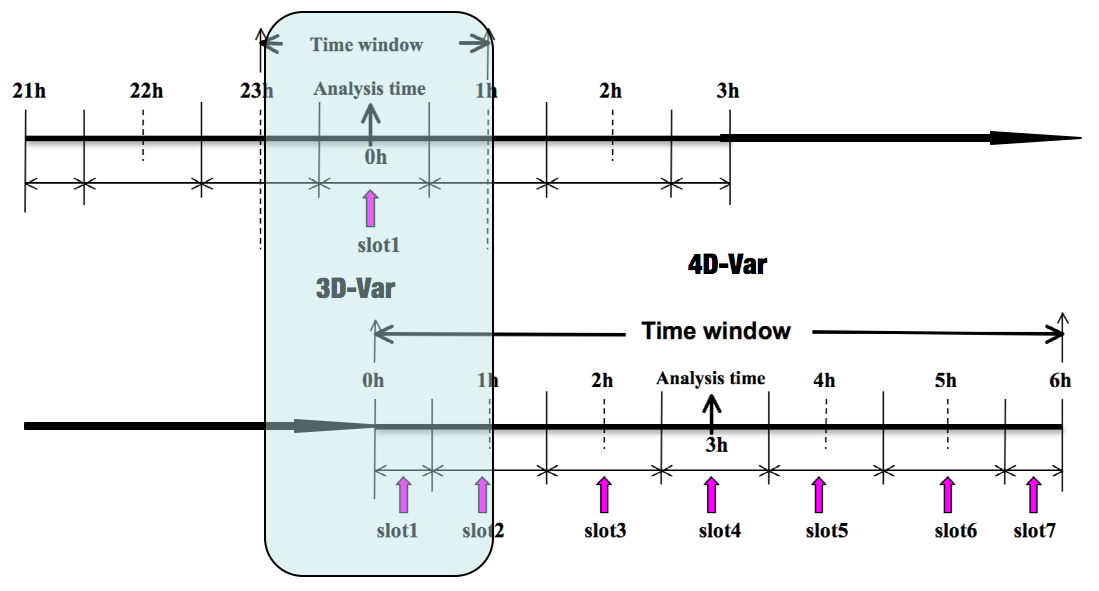
\includegraphics[scale=0.25]{obs_3dvar} \pause
\vspace {-13.61em} 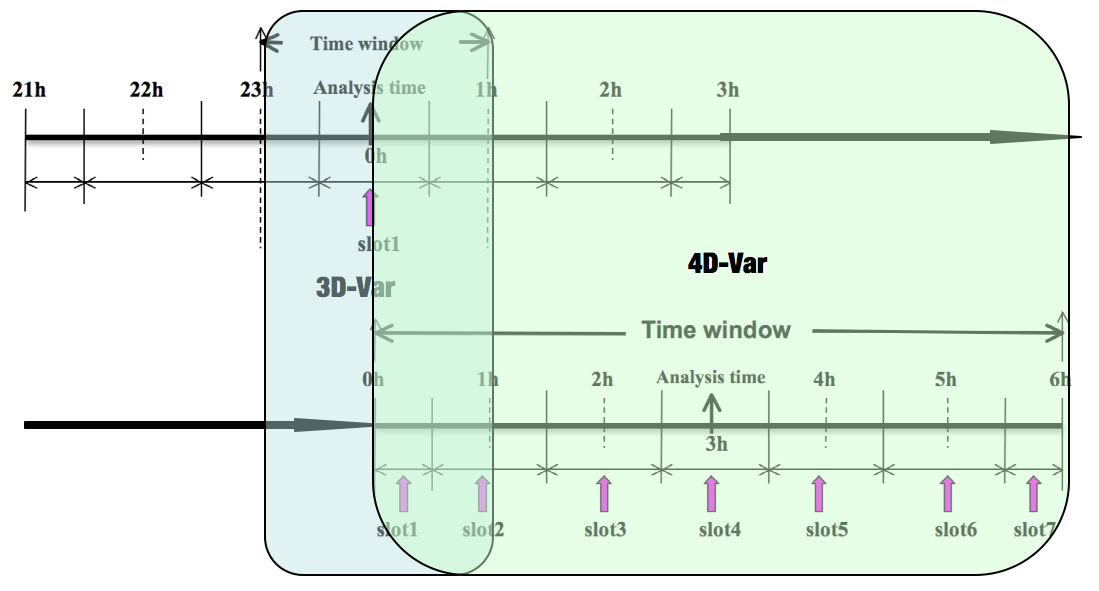
\includegraphics[scale=0.25]{obs_4dvar}
\end{center} 
}
\end{comment}

%%%%%%%%%%%%%%%%%%%%%%%%%
\section{Applications}

\begin{comment}
\frame{
\begin{columns}[c]
\column{5cm}
\includemovie[
  controls,autoresume,poster,
  text={\small(Loading boundarylbcnojcdf.mpeg)}
]{6.0cm}{7.5cm}{boundarylbcnojcdf.mpeg}
\column[c]{3.5cm}
\begin{block}{Remarks}
\tiny{Forecasted 500mb T difference \\(DA forecast - reference forecast)}
\begin{itemize}
	\item {\color{red}$\star$} is the location of obs. at the ending time (6h).
	\item \tiny{JcDF is {\color{red}turned off}}
	\item \tiny{LBC control is turned on}
	\item \tiny{Noise development dominate the domain, the perturbation development is totally different, hard to see the impact of boundary.}
\end{itemize}
\end{block}
\end{columns}
}
\end{comment}

\subsection{OSSE Experiments}

\frame{
\frametitle{Radar radial wind data assimilation}
\begin{itemize}
	\item \small{TRUTH ----- Initial condition from TRUTH (13-h forecast initialized at 	   
                           2002061212Z from AWIPS 3-h analysis) run cutted by ndown, 	     
                           boundary condition from NCEP GFS data.} \pause
	\item \small{NODA -----  Both initial condition and boundary condition from NCEP GFS data.}\pause
	\item \small{3DVAR -----3DVAR analysis at 2002061301Z used as the initial condition, and  
                           boundary condition from NCEP GFS. Only Radar radial velocity at  
                           2002061301Z assimilated (total data points = 97,033), 3 outer loops.}\pause
	\item \small{4DVAR ----- 4DVAR analysis at 2002061301Z used as initial condition, and 
                           boundary condition from NCEP GFS. The radar radial velocity at 4  
                           times: 200206130100, 05, 10, and 15, are assimilated (total
                           data points = 384,304), 1 outer loop.}
\end{itemize}
}

\frame{
\frametitle{OSSE 3rd hour precipitation simulation}
\begin{tabular}{l r}
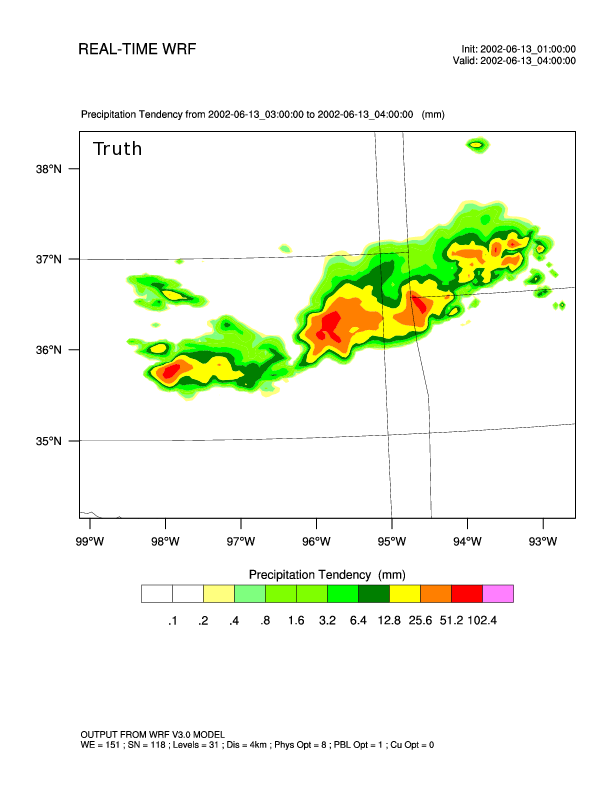
\includegraphics[scale=0.20, trim=1 240 3 100, clip]{radar_truth} & 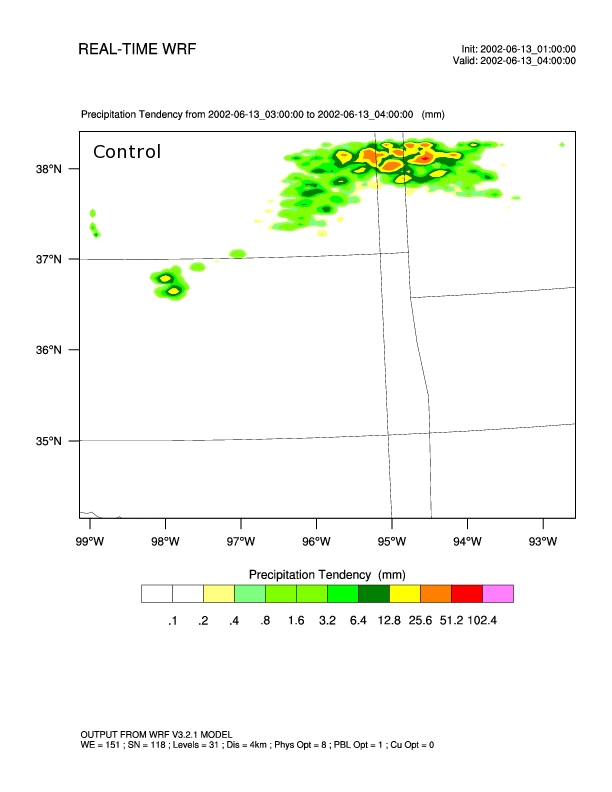
\includegraphics[scale=0.20, trim=1 240 3 100, clip]{radar_control} \\
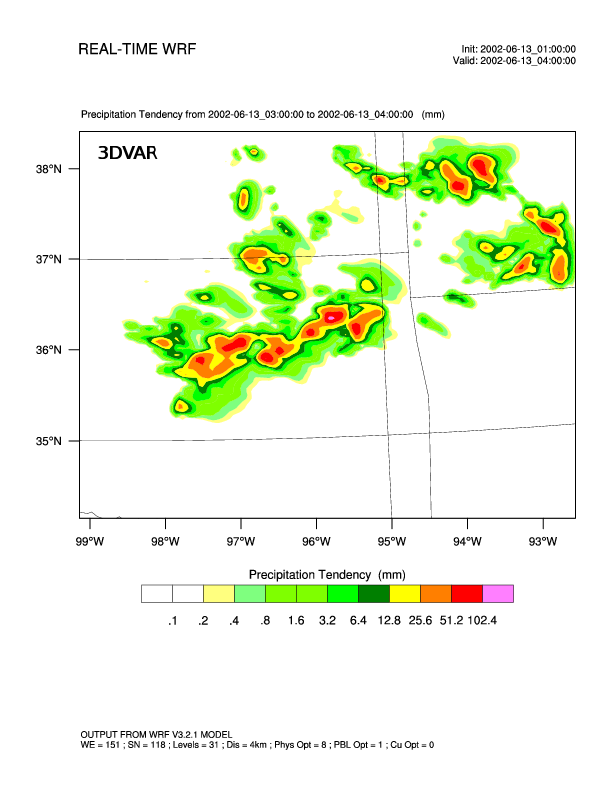
\includegraphics[scale=0.20, trim=1 160 3 130, clip]{radar_3dvar} & 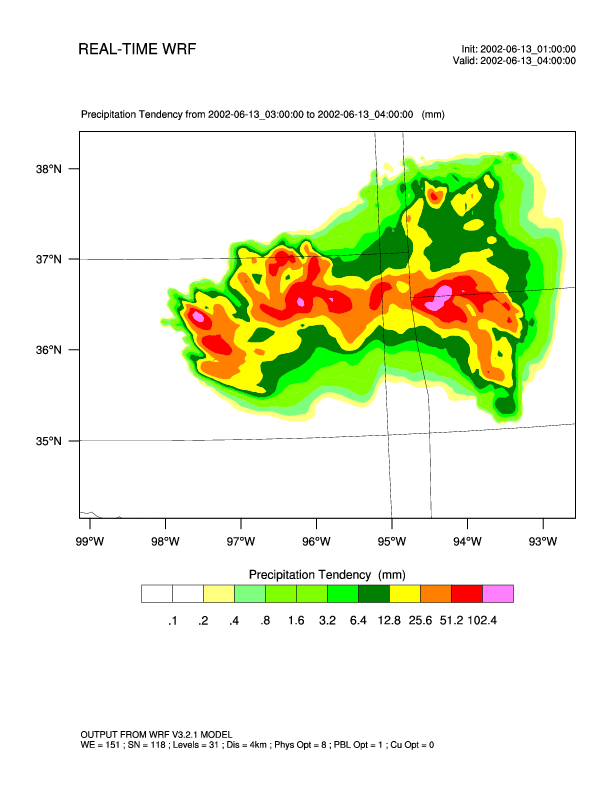
\includegraphics[scale=0.20, trim=1 160 3 130, clip]{radar_4dvar}
\end{tabular}
}

\begin{comment}
\frame{
\frametitle{Remarks}
\begin{itemize}
	\item Obviously, 4DVar reproduce the best squall line precipitation band.\pause
	\item However, the coverage and intensity of the precipitation are more than the observation.
\end{itemize}
}
\end{comment}

\frame{
\frametitle{Precipitation assimilation}
\begin{itemize}
	\item WRFPLUS includes the TL and AD of:
	\begin{itemize}
		\item Large scale condensation (mp\_physics=98)
		\item CUDU cumulus scheme (cu\_physics=98)
	\end{itemize}
	\item An OSSE experiment are conducted to verify the capability
	\item 2010-09-11-00 +6h precipitation (IC and BC come from +12h forecast from 2010-09-10-12 NCEP FNL)
\end{itemize}
}

\frame{
\frametitle{OSSE exp. flowchart}
\begin{center}
\includegraphics[scale=0.35]{rainobs/flowchart}
\end{center} 
}

\frame{
\frametitle{Minimization}
\begin{tabular}{c c}
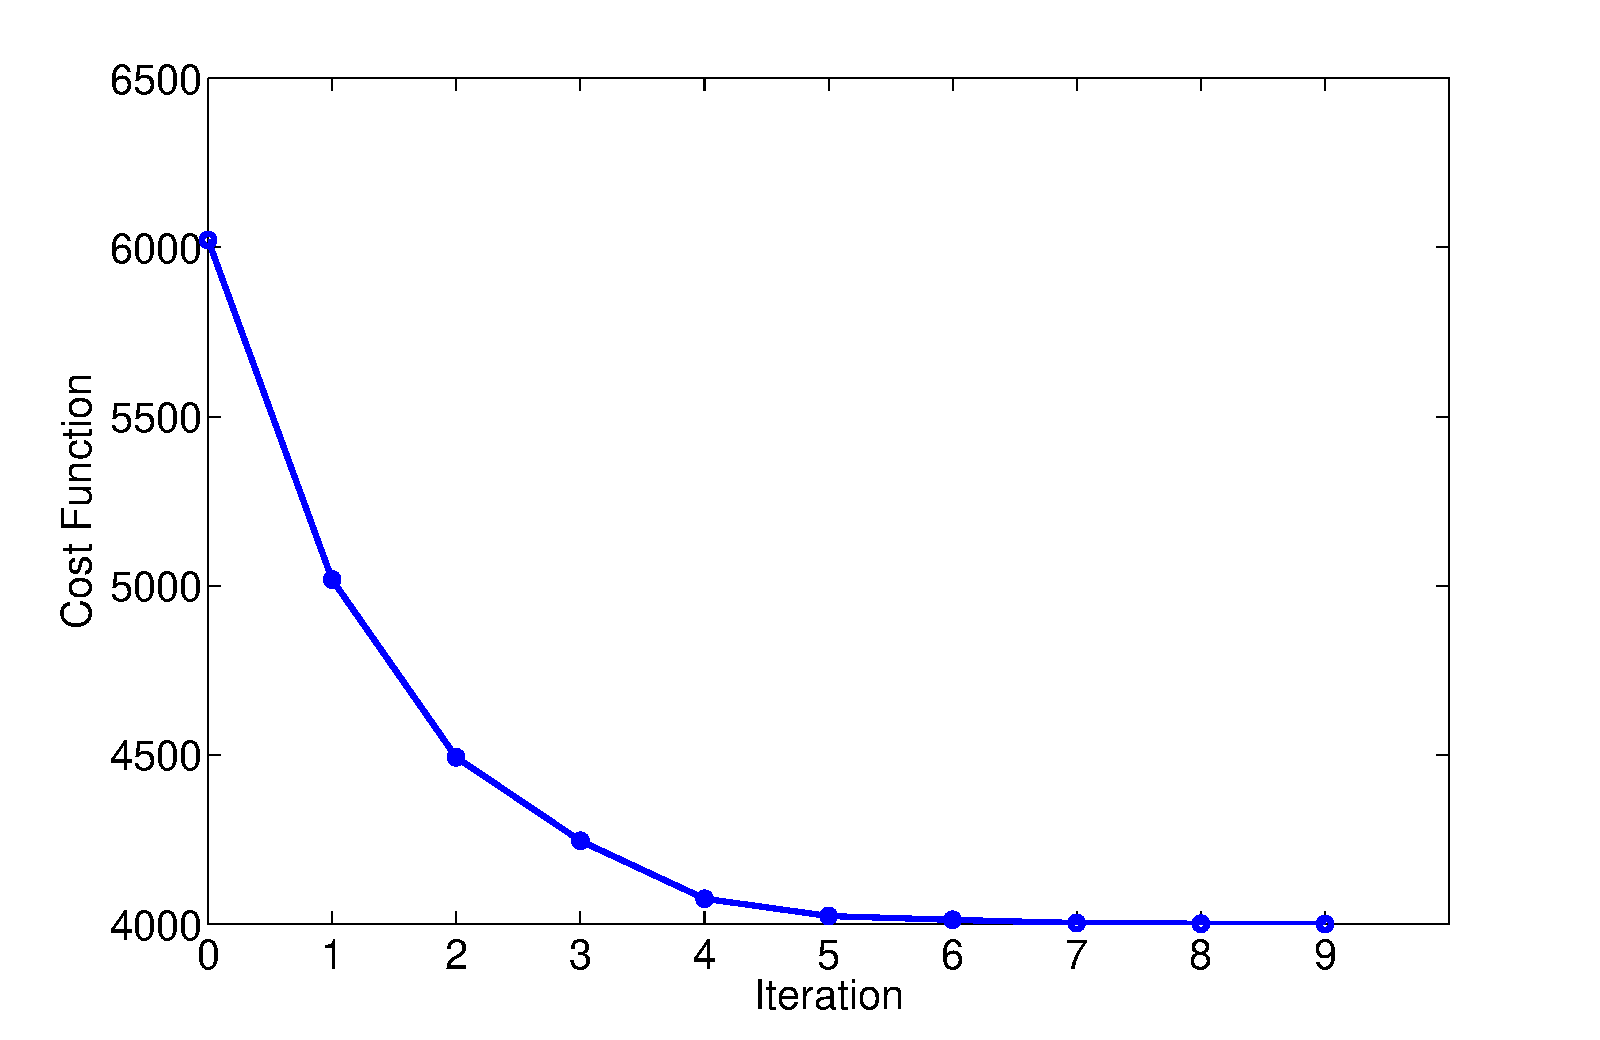
\includegraphics[scale=0.42]{rainobs/cost} & 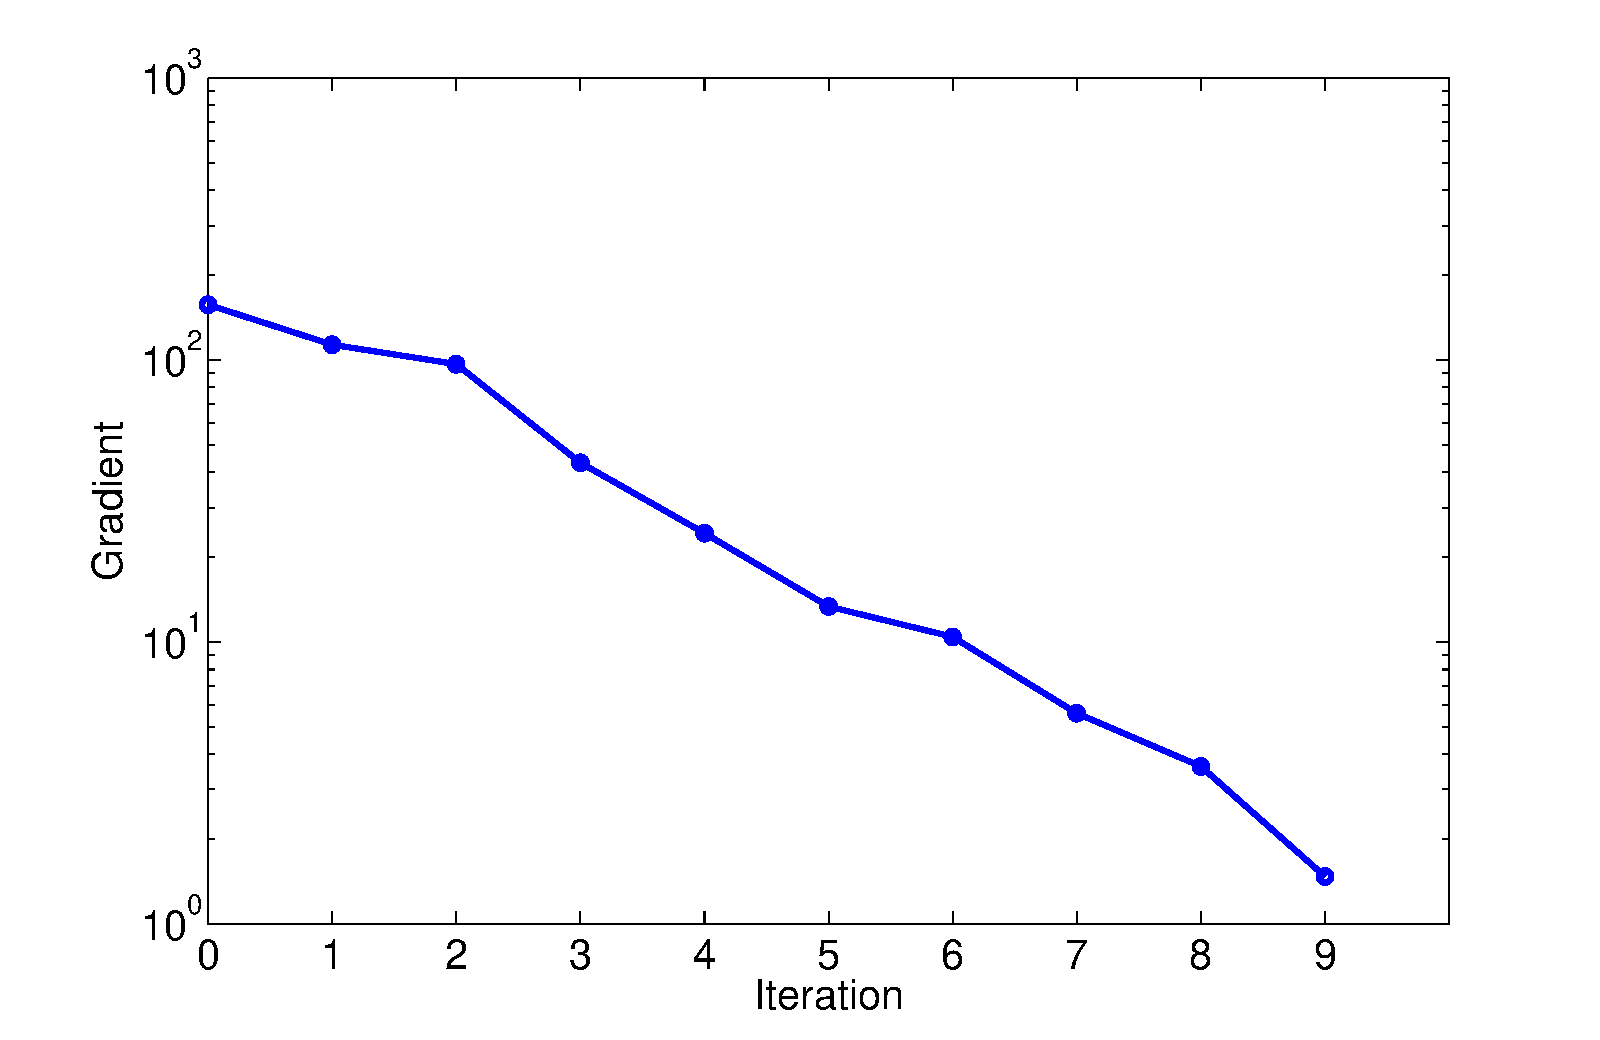
\includegraphics[scale=0.42]{rainobs/grad}
\end{tabular}
}

\frame{
\frametitle{2010091100 +6h simulated accumulated precipitation forecast, sampled by 2066 metar station+random error}
\begin{center}
\includegraphics[page=2, scale=0.4,  trim=25 50 25 150, clip]{rainobs/rain_00-06} 
\end{center}
}

\frame{
\frametitle{+6h total precipitation simulations}
\begin{tabular}{c c}
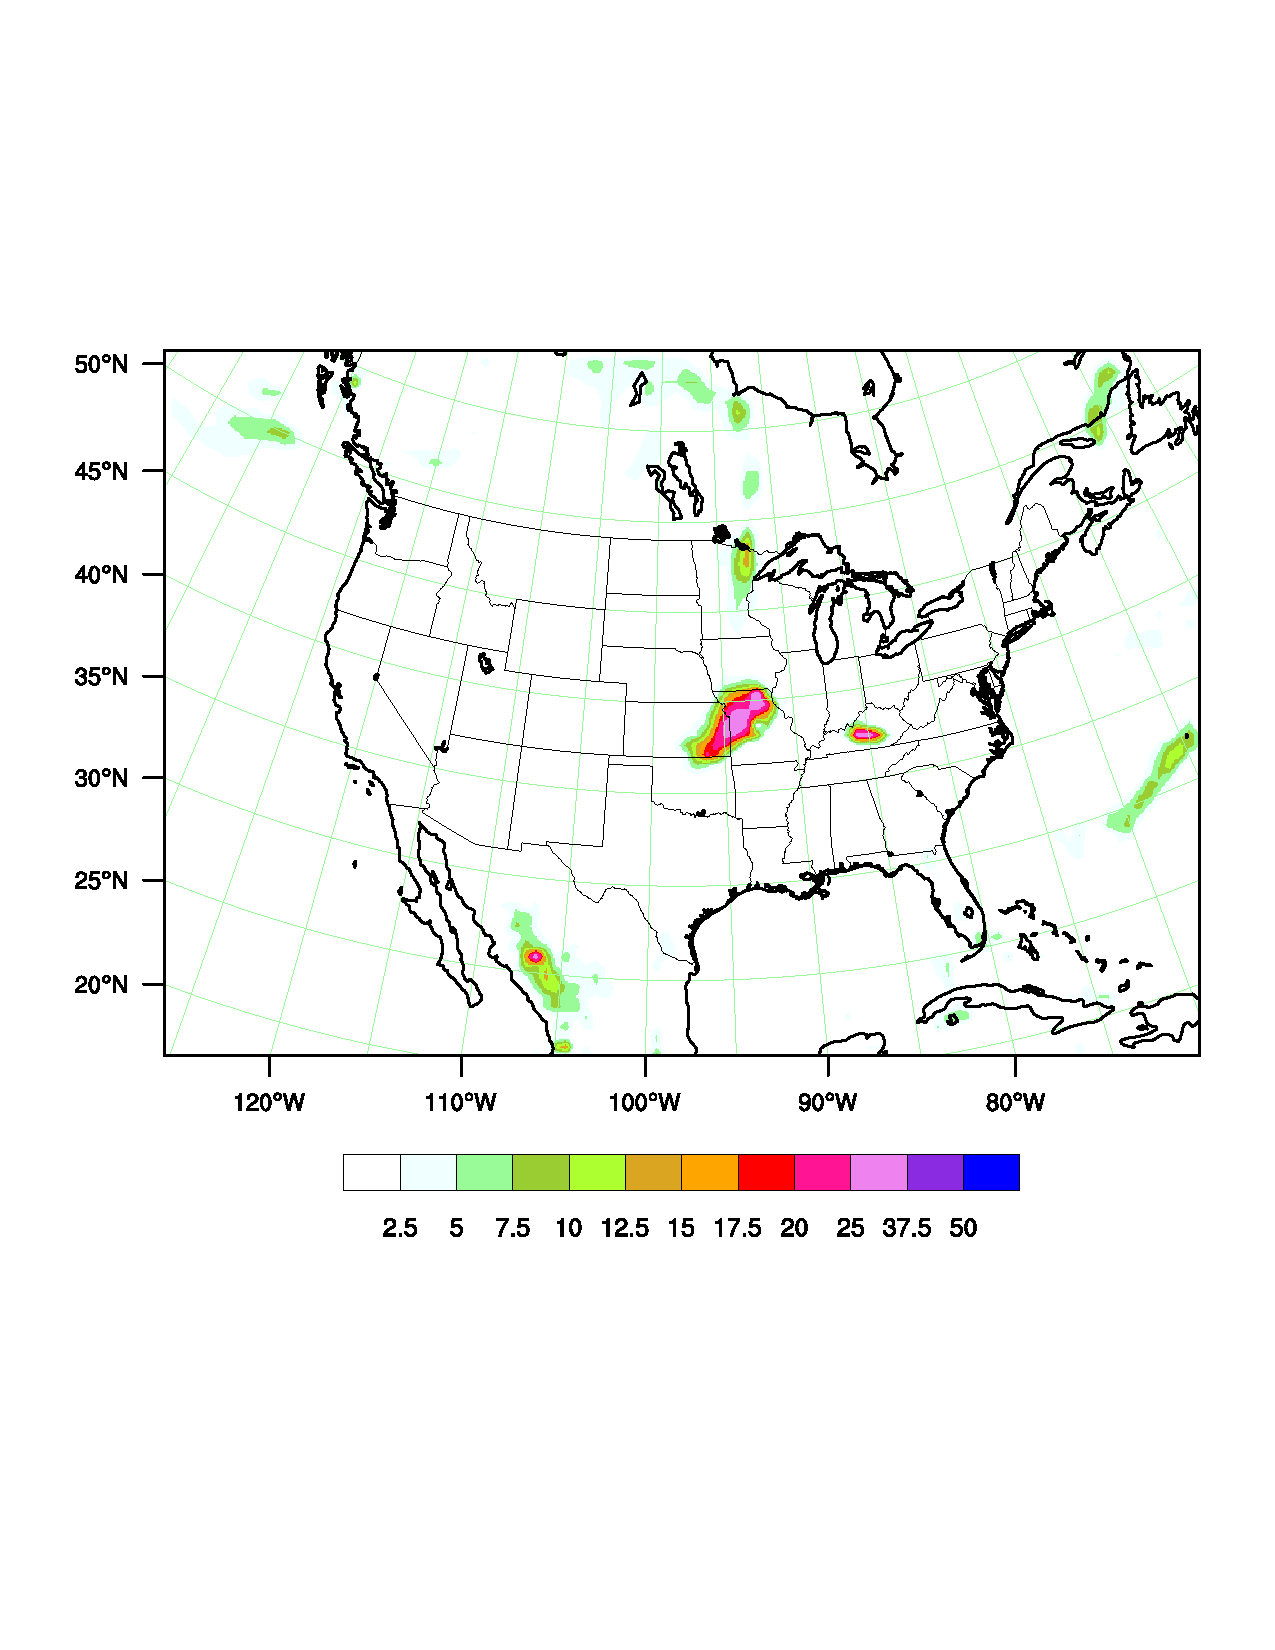
\includegraphics[scale=0.23, trim=30 180 30 100, clip]{rainobs/control_00-06} & 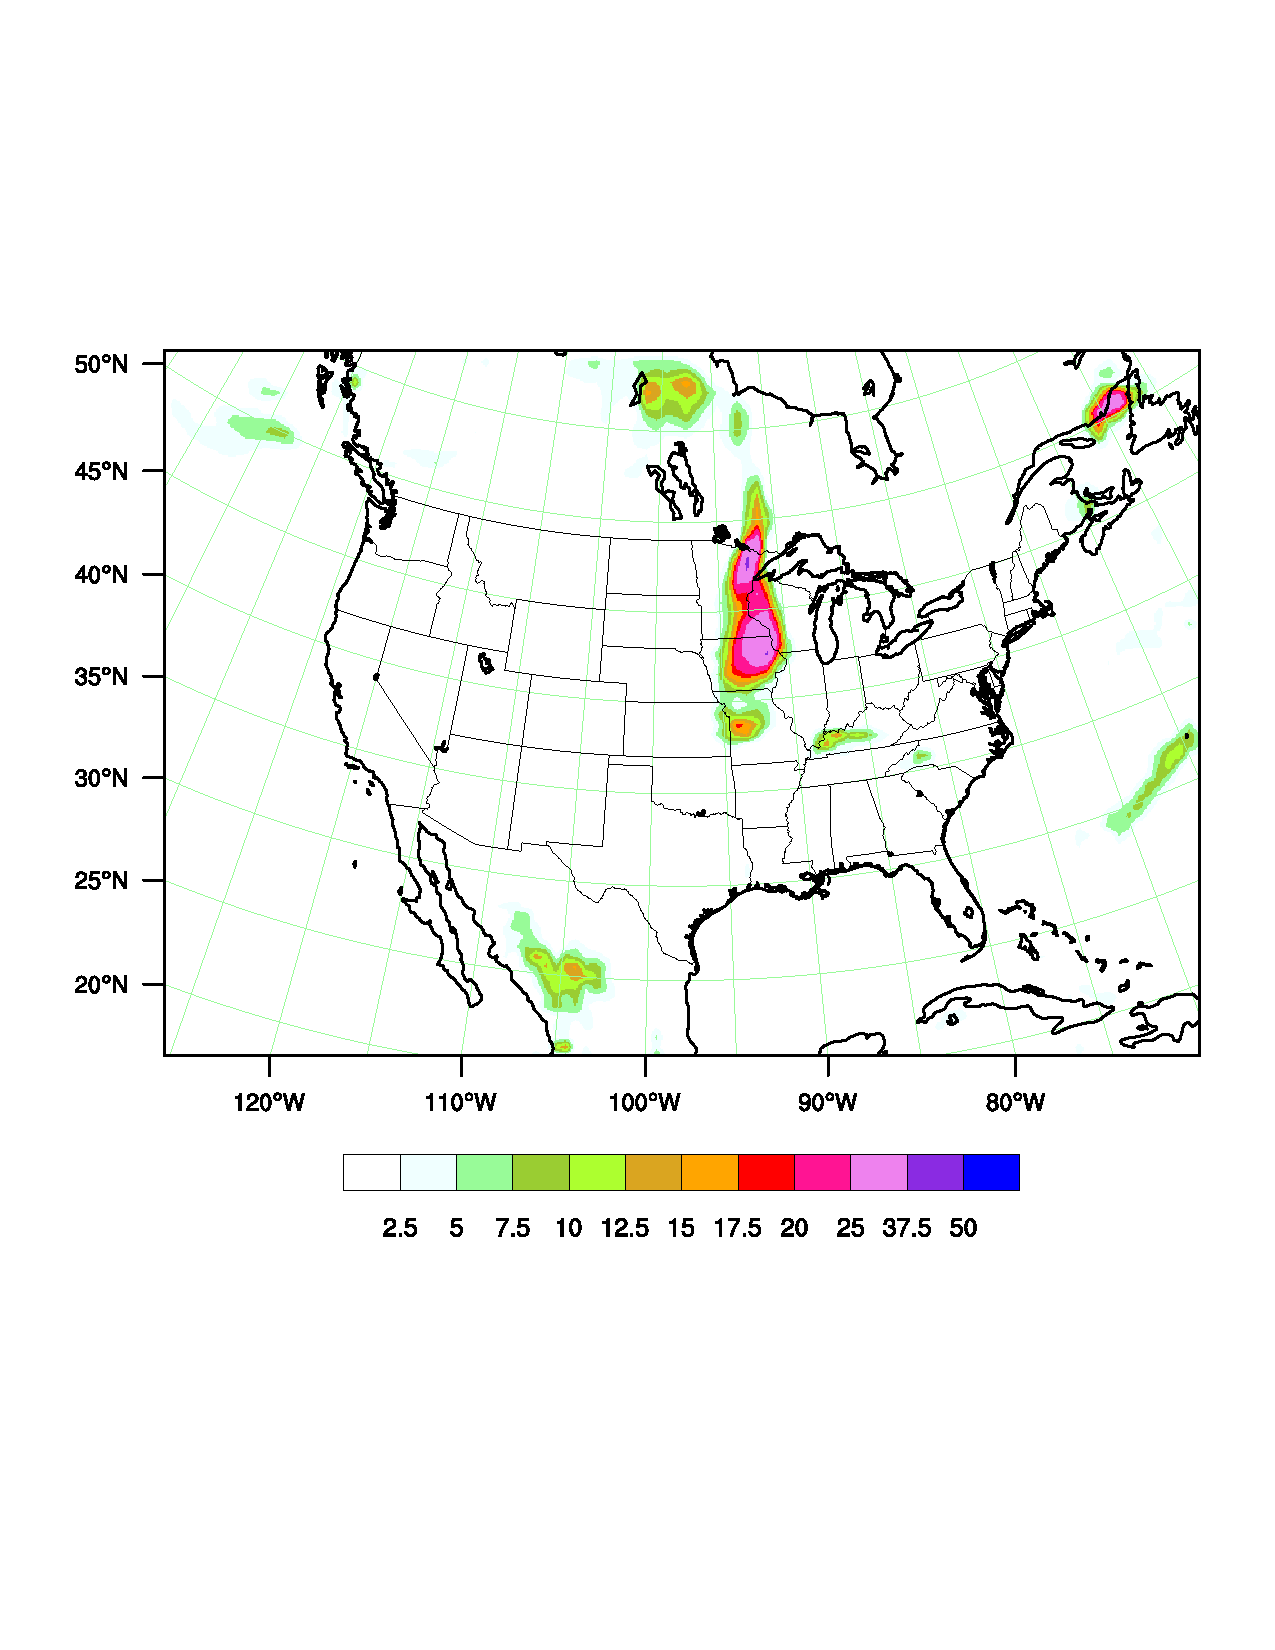
\includegraphics[scale=0.23, trim=30 180 3 100, clip]{rainobs/asrain_00-06} \\
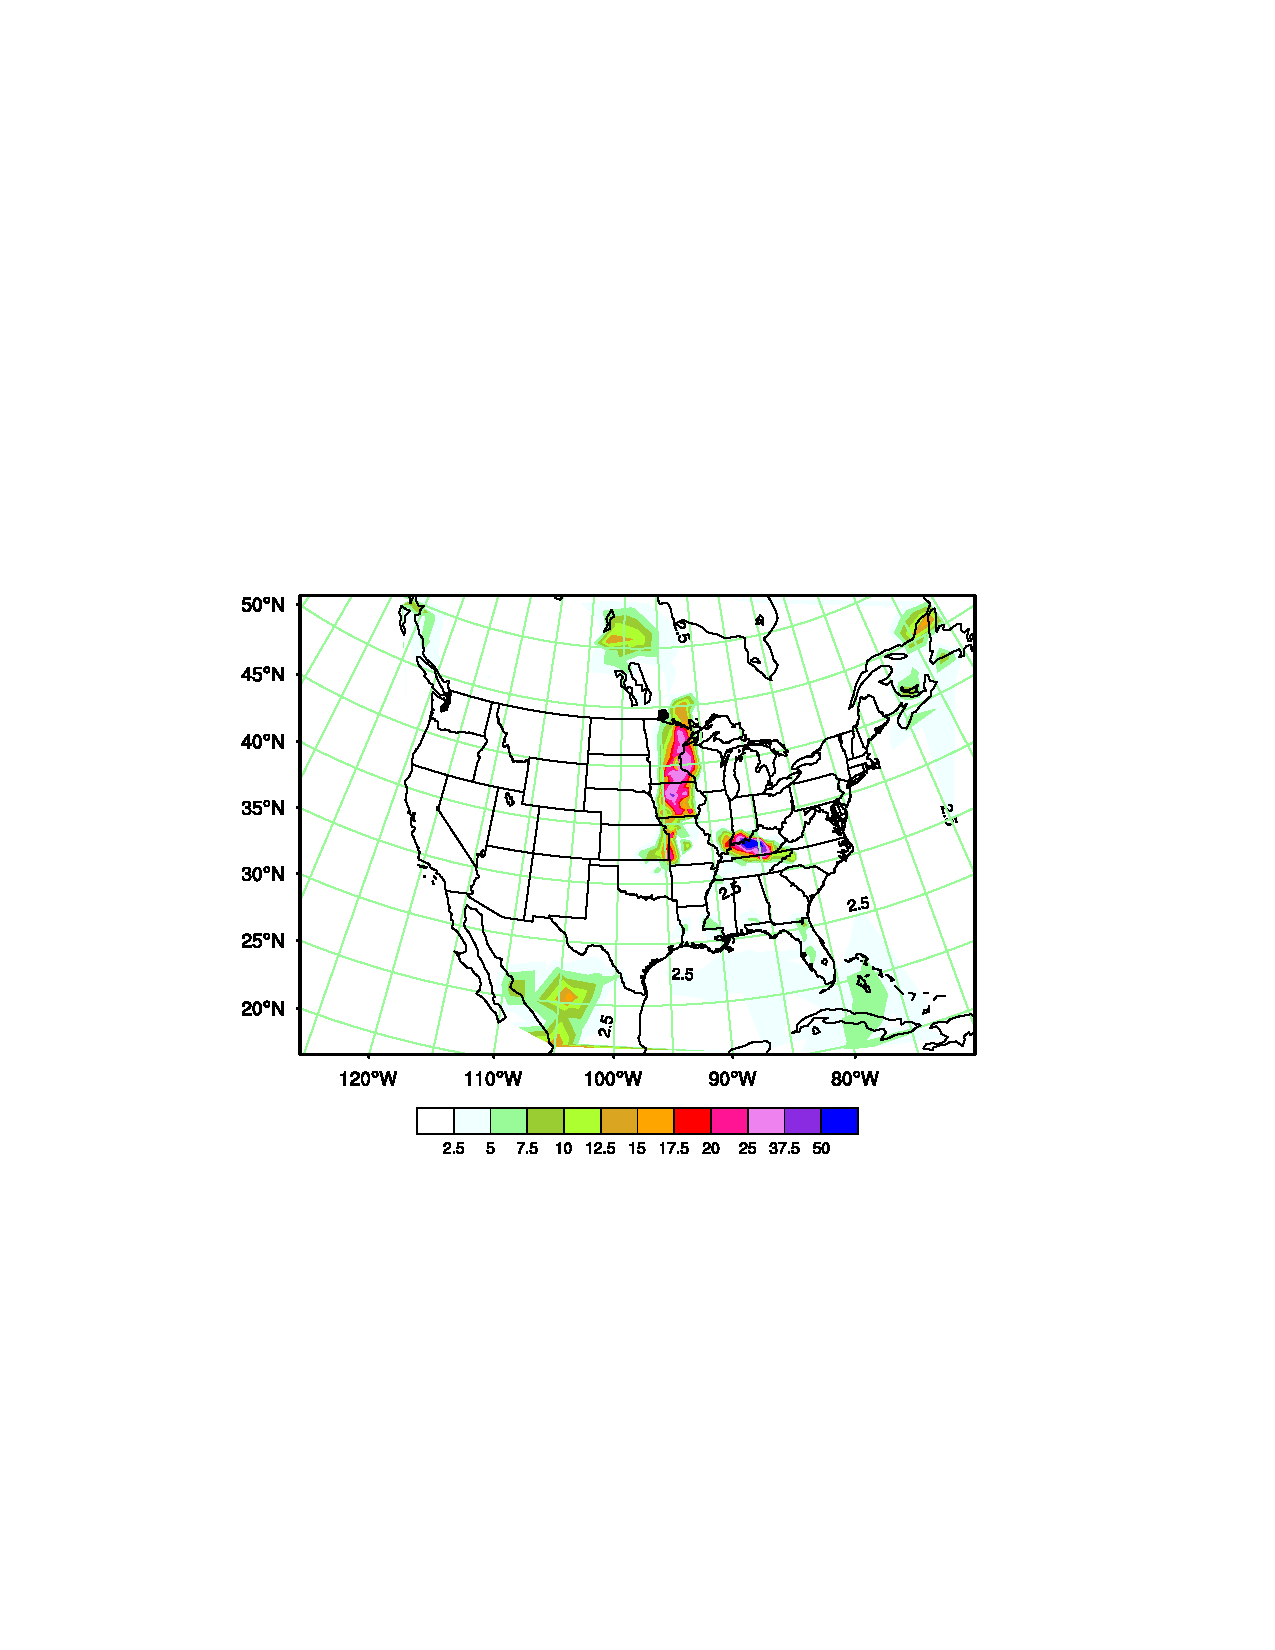
\includegraphics[scale=0.30, trim=1 160 3 270, clip]{rainobs/rain_00-06} 
\end{tabular}
}

\frame{
\frametitle{Conclusion}
\begin{itemize}
	\item Preliminary OSSE experiments confirm that precipitation assimilation can effectively reduce the spin-up for the first 6h. \pause 
	\item The convergence of minimization looks good. \pause
	\item Real cases exp. will be conducted to further check the capability.
\end{itemize}
}


\subsection{Real cases}

\frame{
\frametitle{1999 Denmark Storm}
\begin{itemize}
	\item \tiny{Grids: 120x90x45L}
	\item Resolution: 30km
	\item Period: 1999120100-1999120512 @0Z,6Z,12Z,18Z
	\item Prepbufr conventional observational data
	\item Start from NCEP FNL, full cycle run
	\item 48h forecasts from FG (control), 3dvar, 4dvar and 4dvar\_lbc (4dvar with LBC control)
	\item Verified against ECMWF re-analysis
\end{itemize}
\begin{center}
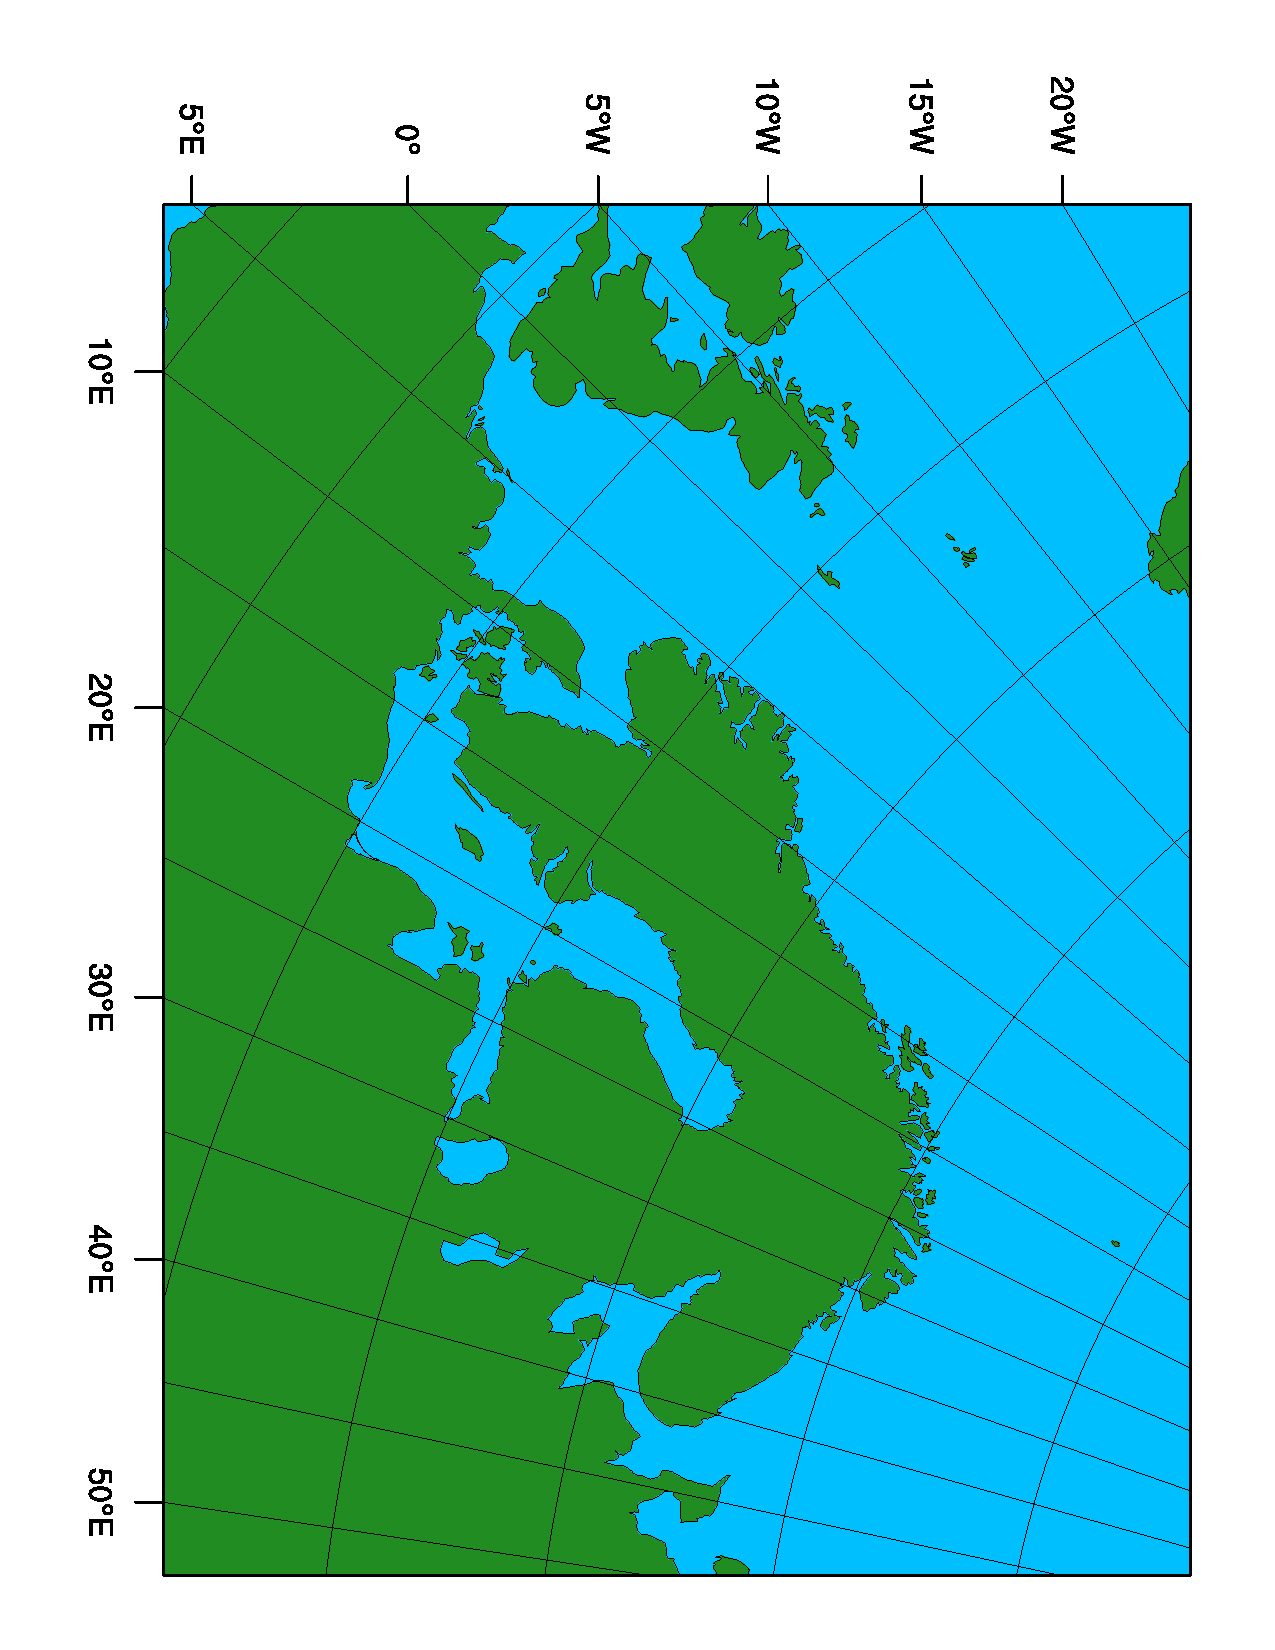
\includegraphics[scale=0.25, trim=0 0 0 0, clip, angle=90]{denmark_domain.pdf} 
\end{center}
}

\frame{
\frametitle{Averaged RMSE of 12H forecast verification}
\begin{center}
\includegraphics[scale=0.30, trim=0 100 0 55, clip]{denmark/Profile_RMSE-hr12.pdf}
\end{center}
}

\frame{
\frametitle{Averaged RMSE of 24H forecast verification}
\begin{center}
\includegraphics[scale=0.30, trim=0 100 0 55, clip]{denmark/Profile_RMSE-hr24.pdf}
\end{center}
}

\frame{
\frametitle{Averaged RMSE of 36H forecast verification}
\begin{center}
\includegraphics[scale=0.30, trim=0 100 0 55, clip]{denmark/Profile_RMSE-hr36.pdf}
\end{center}
}

\frame{
\frametitle{Averaged RMSE of 48H forecast verification}
\begin{center}
\includegraphics[scale=0.30, trim=0 100 0 55, clip]{denmark/Profile_RMSE-hr48.pdf}
\end{center}
}

\frame{
\begin{center}
Comparison of the Exp. of 4D-Var and Exp. 4D-Var with LBC control
\end{center}
}

\frame{
\frametitle{Averaged RMSE of 12H forecast verification}
\begin{center}
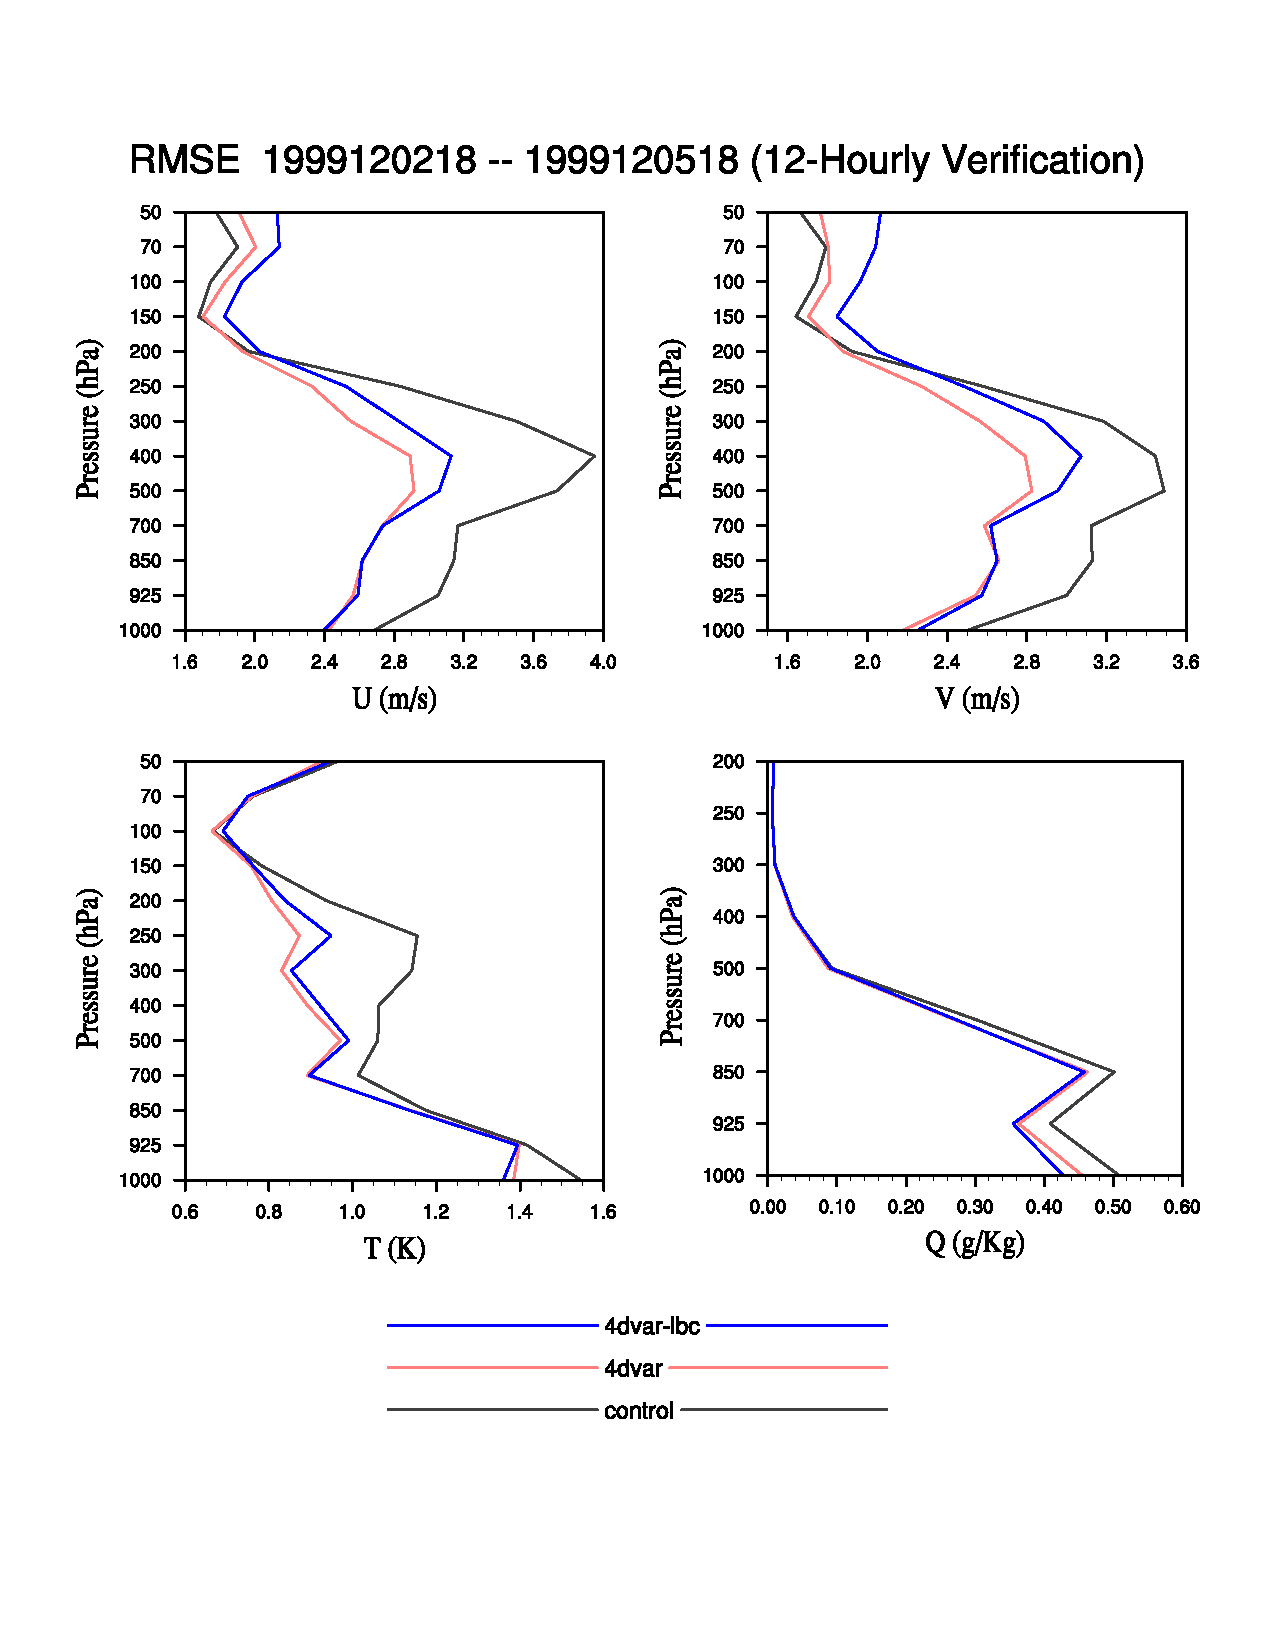
\includegraphics[scale=0.30, trim=0 100 0 55, clip]{denmark/Profile_RMSE-hr12_lbc.pdf}
\end{center}
}

\frame{
\frametitle{Averaged RMSE of 24H forecast verification}
\begin{center}
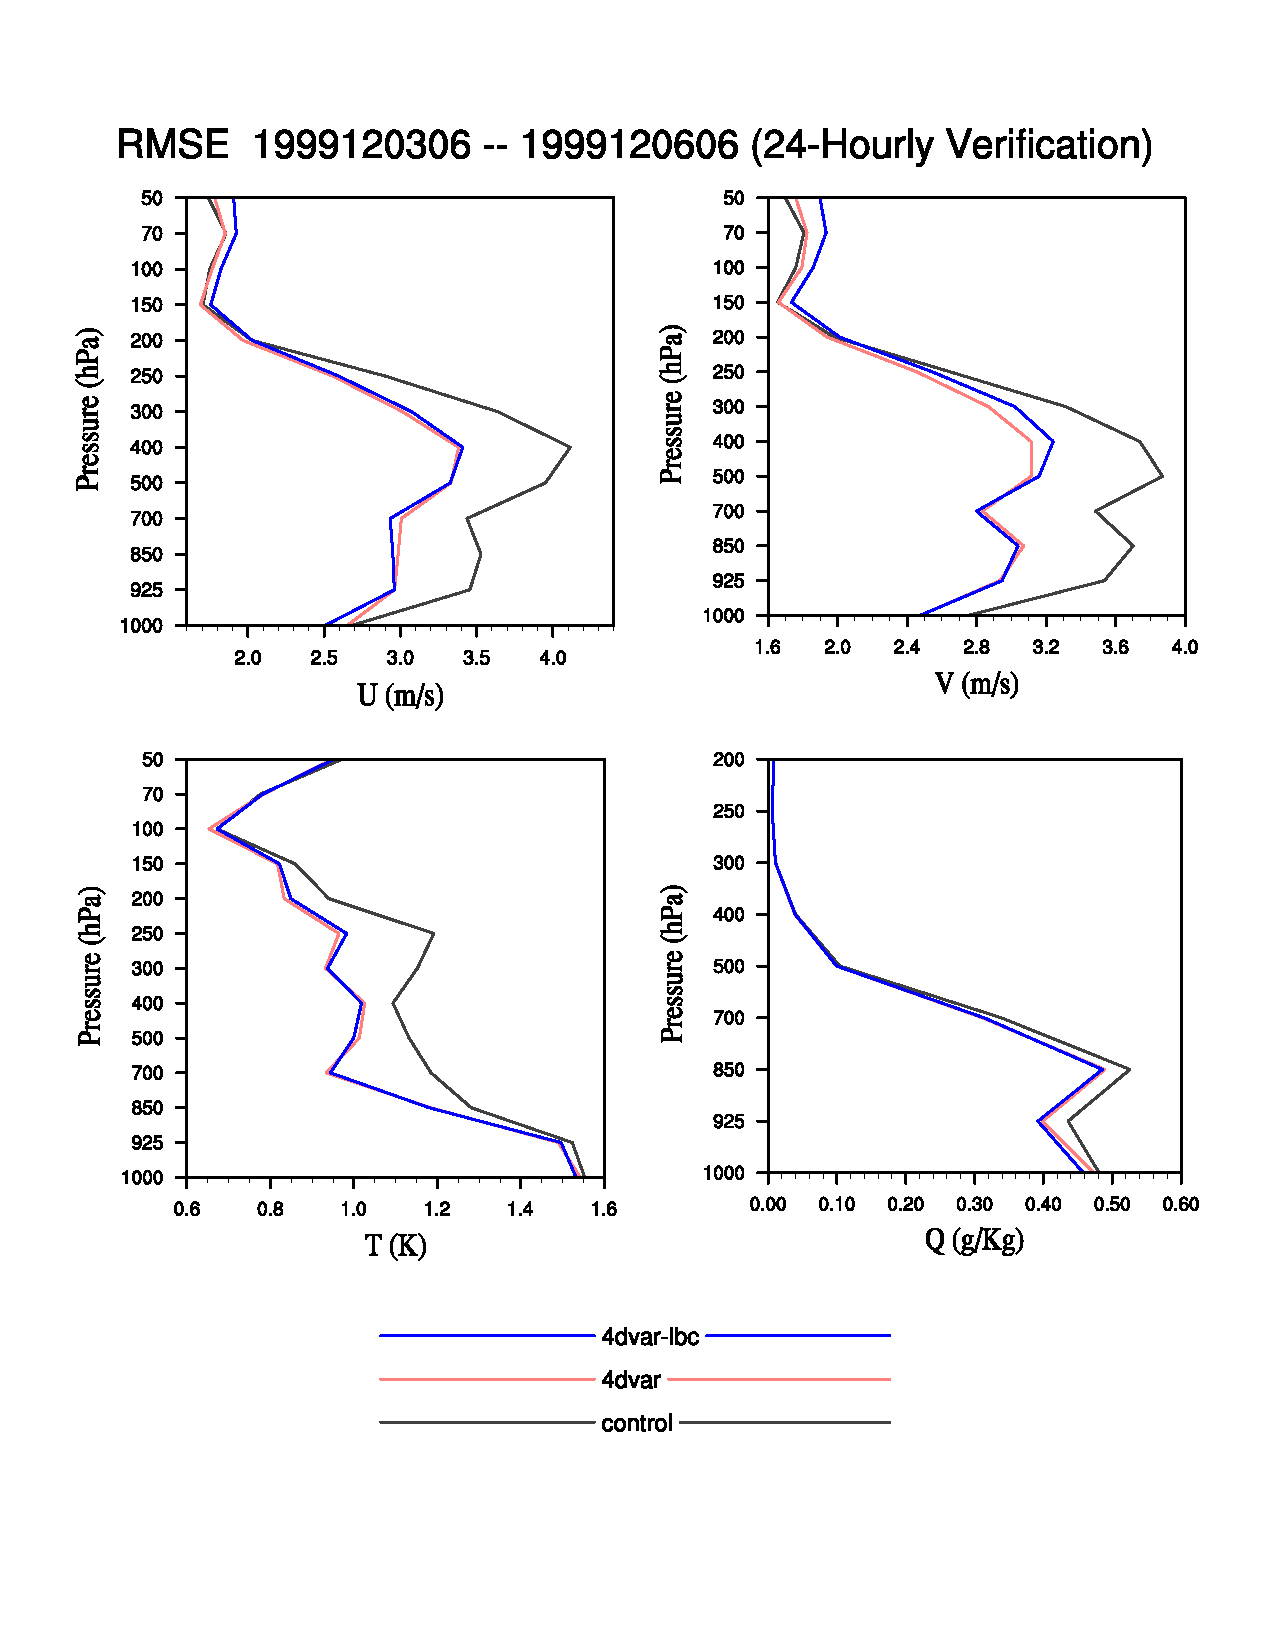
\includegraphics[scale=0.30, trim=0 100 0 55, clip]{denmark/Profile_RMSE-hr24_lbc.pdf}
\end{center}
}

\frame{
\frametitle{Averaged RMSE of 36H forecast verification}
\begin{center}
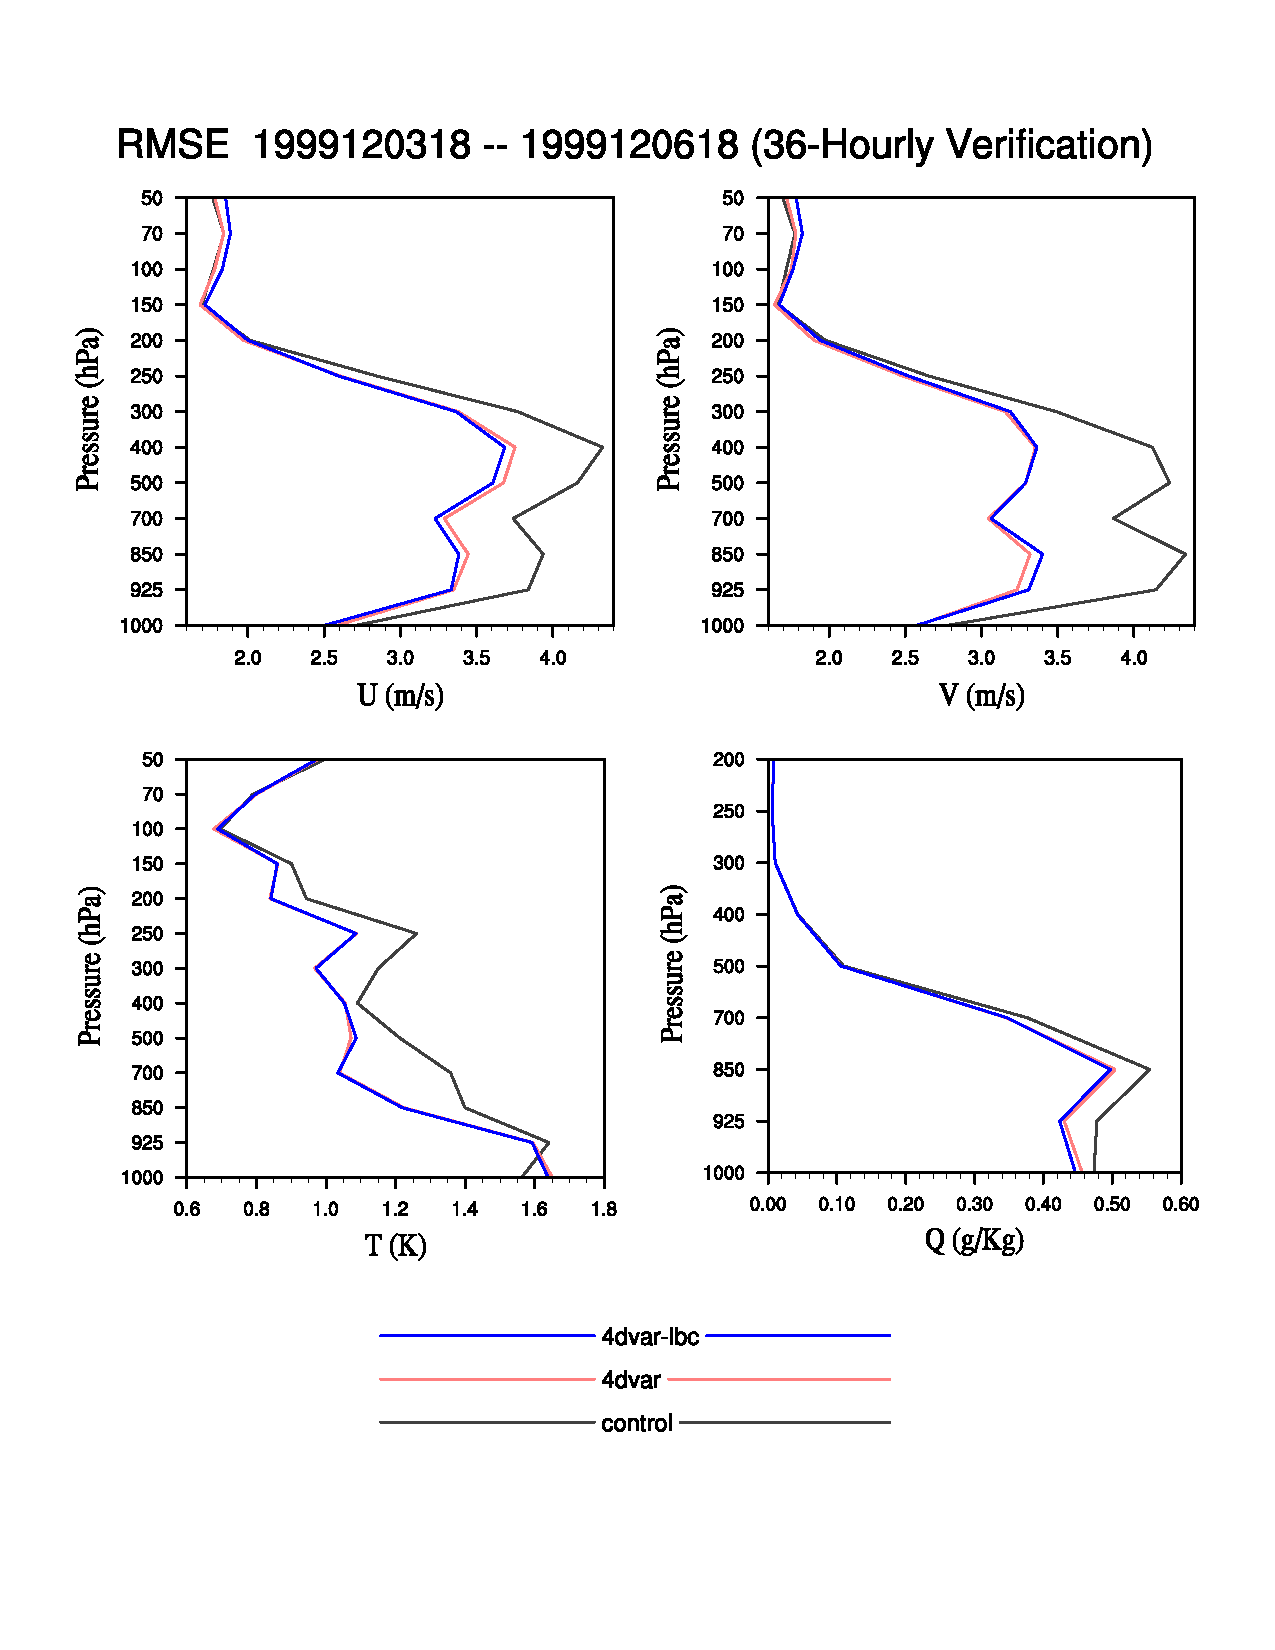
\includegraphics[scale=0.30, trim=0 100 0 55, clip]{denmark/Profile_RMSE-hr36_lbc.pdf}
\end{center}
}

\frame{
\frametitle{Averaged RMSE of 48H forecast verification}
\begin{center}
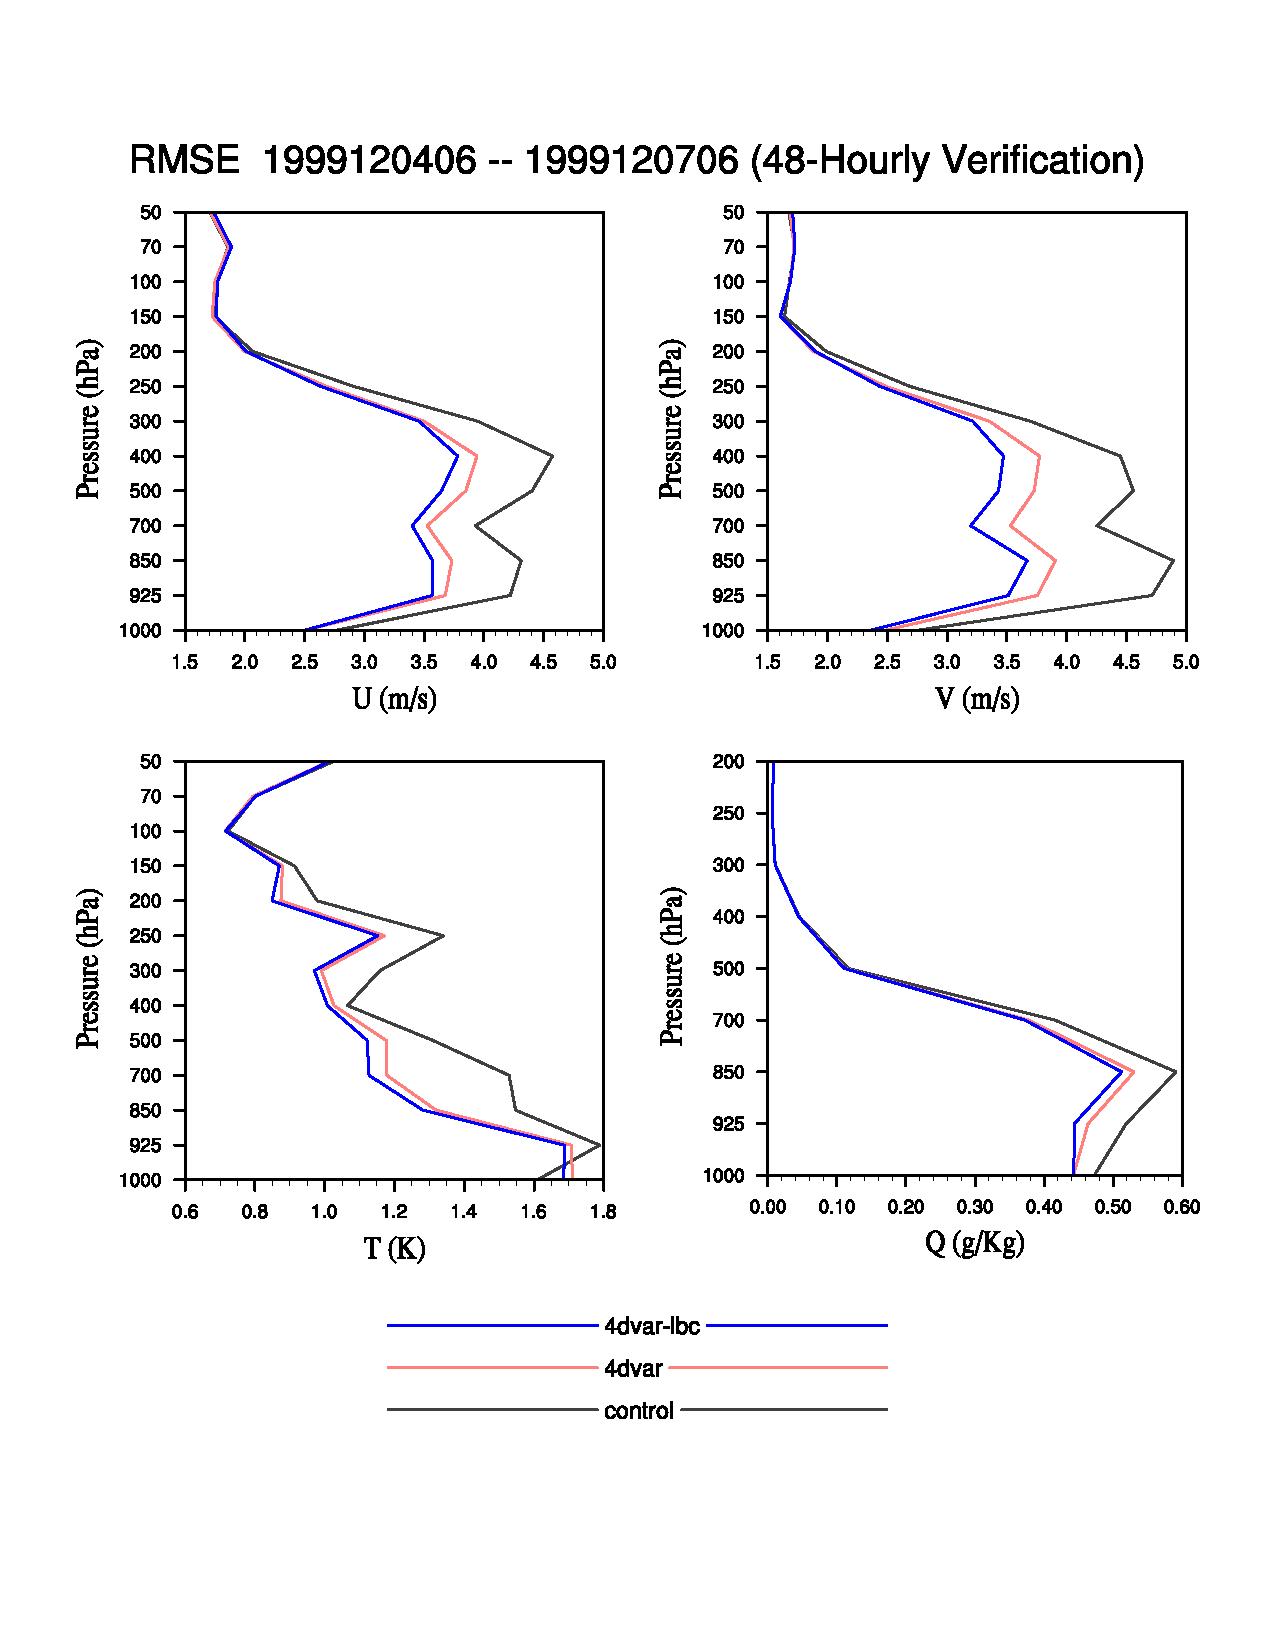
\includegraphics[scale=0.30, trim=0 100 0 55, clip]{denmark/Profile_RMSE-hr48_lbc.pdf}
\end{center}
}

\frame{
\frametitle{Conclusion}
\begin{itemize}
	\item This five days (20 cycles) experiments show that the 4DVAR outperforms 3DVAR significantly. \pause 
	\item 4DVAR-LBC outperforms 4DVAR from 24h forecast. Especially, 4DVAR-LBC outperforms 4DVAR significantly on 48h forecast. \pause
	\item From 0-24h forecast, 4DVAR-LBC doesn�t show advantages compared to 4DVAR, the reason is unknown so far. One assumption is that the degradation during the first 24h is due to the noises introduced by LBC control (Gustafsson, 1998), model needs time to spin-up. \pause
	\item Plan to run one month experiment with digital filter as weak constraint to further confirm.
\end{itemize}
}

\frame{
\frametitle{CWB OP23 Partial Cycle}
\begin{center}
\includegraphics[scale=0.40, trim=0 200 150 5, clip]{cwb/Partial_cycle_origin}
\end{center}
}

\frame{
\frametitle{CWB OP23 Partial Cycle 4D-Var Ver. 0}
\begin{center}
\includegraphics[scale=0.40, trim=0 200 150 5, clip]{cwb/Partial_cycle_4dvar_v0}
\end{center}
\begin{itemize}
	\item Using 0-6h observations in $3^{rd}$ DTG
	\item no DFI initialization in $3^{rd}$ DTG
\end{itemize}
}

\frame{
\frametitle{CWB OP23 Domains}
\begin{center}
\includegraphics[scale=0.30, trim=90 0 60 0, clip, angle=90]{cwb/wps_show_dom3}
\end{center}
}

\frame{
\frametitle{CWB OP23 4D-Var Ver. 0 Domain}
\begin{center}
\includegraphics[scale=0.30, trim=90 0 60 0, clip, angle=90]{cwb/wps_show_dom}
\end{center}
\begin{itemize}
	\item Analysis/forecast times: 00 and 12UTC of 2010-12-01---12-15 
	\item 0-48h forecast verified against ECMWF reanalysis
\end{itemize}
}

\frame{
\frametitle{CWB OP23 4D-Var Ver. 0 Verification 00h}
\begin{center}
\includegraphics[scale=0.30, trim=0 0 0 40, clip]{cwb/Profile_RMSE-hr0}
\end{center}
}

\frame{
\frametitle{CWB OP23 4D-Var Ver. 0 Verification 06h}
\begin{center}
\includegraphics[scale=0.30, trim=0 0 0 40, clip]{cwb/Profile_RMSE-hr6}
\end{center}
}

\frame{
\frametitle{CWB OP23 4D-Var Ver. 0 Verification 12h}
\begin{center}
\includegraphics[scale=0.30, trim=0 0 0 40, clip]{cwb/Profile_RMSE-hr12}
\end{center}
}

\frame{
\frametitle{CWB OP23 4D-Var Ver. 0 Verification 24h}
\begin{center}
\includegraphics[scale=0.30, trim=0 0 0 40, clip]{cwb/Profile_RMSE-hr24}
\end{center}
}

\frame{
\frametitle{CWB OP23 4D-Var Ver. 0 Verification 36h}
\begin{center}
\includegraphics[scale=0.30, trim=0 0 0 40, clip]{cwb/Profile_RMSE-hr36}
\end{center}
}

\frame{
\frametitle{CWB OP23 4D-Var Ver. 0 Verification 48h}
\begin{center}
\includegraphics[scale=0.30, trim=0 0 0 40, clip]{cwb/Profile_RMSE-hr48}
\end{center}
}

\frame{
\frametitle{Proposed CWB OP23 Partial Cycle 4D-Var Ver. 1}
\begin{center}
\includegraphics[scale=0.40, trim=0 200 150 5, clip]{cwb/Partial_cycle_4dvar_v1}
\end{center}
\begin{itemize}
	\item Using 4D-Var in $1^{st}$ and $2^{nd}$ DTGs, no cut-off time.
	\item Using 3D-Var in $3^{rd}$ DTG.
	\item Using time window from 0--6h, fully takes advantage of the observations.
\end{itemize}
}

\frame{
\frametitle{Parallel timing/speedup of CWB OP23 on NCAR bluefire}
Domain size: 222x128x45L, 45km\\
On IBM bluefire,  xlf V13.01, cost of 5 iterations (40 iteration to converge) \\ 
~\\
~\\
\begin{center}
\begin{tabular}{c | c  | l}
\hline
Processors & Perfect &  Total \\
\hline \hline
32 & 1 & 97m/1.0 \\
64 & 2 &  43m/2.26 \\
128 & 4 &  26m/3.73\\
256 & 8 &  19m/5.1\\
\hline
\end{tabular}
\end{center}
}

%%%%%%%%%%%%%%%%%%%%%%%%%%%%%%%%%
\section{Summary}

\frame{
\frametitle{Summary}
\begin{itemize}
	\item The single executable WRF 4D-Var system was developed and has showed promising performance. \pause 
	\item The new WRF 4D-Var system has the capability to assimilate conventional observational data (little\_r or prepbufr format),radiance in bufr format and radar data. \pause
	\item The new WRF 4D-Var system is able to consider lateral boundary condition as control variable and digital filter can be used as a weak constraint to suppress the high frequency noise. \pause
	\item Multiple outer loops for 4D-Var.
\end{itemize}
}

\frame{
\frametitle{Future Developments in 2012}
\begin{itemize}
	\item Add more physics packages into WRFPLUS: radiation scheme (GSFC), surface physics scheme to improve surface observation assimilation.  \pause
	\item Multi-incremental 4D-Var configuration.\pause
	\item Add precipitation observation to the forcing term (almost done). \pause
	\item Hybrid-4dvar scheme (wish list)
\end{itemize}
}

\begin{comment}
\begin{frame}[fragile]
\frametitle{Quick Start}
Install WRFPLUS and WRFPLUS
   \begin{itemize}
        	\item WRFPLUS : WRF adjoint and tangent linear codes
		\begin{verbatim}
	         > configure [-d] wrfplus
	         > compile em_real
	         \end{verbatim}
	\item Set the the $WRFPLUS\_DIR$ environmental variable, it will be used in WRFDA compilation
		\begin{verbatim} 
		> setenv WRFPLUS_DIR full_path_of_wrfplus  
		\end{verbatim}
	\item WRFDA
		\begin{verbatim}
		> configure [-d] 4dvar
		> compile all_wrfvar
		\end{verbatim}
    \end{itemize}
\end{frame}

\frame{
\frametitle{Upcoming}
A hand-on tutorial for WRF 4D-Var V3.3 will be presented on June 24, Friday morning 8:30AM-10:00AM
\begin{itemize}
	\item Overview
	\item Installation
	\item Setup
	\item Run
\end{itemize}
}
\end{comment}
%%%%%%%%%%%%%%%%%%%%%%%%%%%%%%%%%%%
\frame{
\begin{center}
~\\
~\\
~\\
~\\
~\\
{\huge{\color{red}Thank You}}\\
~\\
~\\
~\\
~\\
~\\
{\tiny{\color{blue}The NESL Mission is: \\
To advance understanding of weather, climate, atmospheric composition and processes;\\
To provide facility support to the wider community; and, \\
To apply the results to benefit society.\\}}
~\\
{\small{NCAR is sponsored by the National Science Foundation}}
\end{center}
}

\end{document}
